\documentclass[xcolor=dvipsnames,aspectratio=169]{beamer}

% INCLUSIÓN DOS PAQUETES IMPRESCINDIBLES DE IDIOMA E CODIFICACIÓN DE CARACTERE.
\usepackage[T1]{fontenc}
\usepackage[english]{babel}
\usepackage[utf8]{inputenc}
\usepackage{csquotes}

%ACRONYMS para engadir un glosario de acronimos automatizado
% \usepackage[acronyms,nonumberlist,nopostdot,nomain,nogroupskip]{glossaries}
% \input{./acronyms.tex}

% PAQUETES PARA FIGURAS E GRAFICOS
\usepackage{graphicx}
%   \usepackage[pdftex]{graphicx}
  \usepackage{epstopdf}
   \graphicspath{{./img/}}
  % and their extensions so you won't have to specify these with
  % every instance of \includegraphics
   \DeclareGraphicsExtensions{.eps,.pdf,.png,.jpg}   
\usepackage{subfigure}
\usepackage{caption}
\usepackage[inkscapelatex=false]{svg}

%Tikz plots
\usepackage{tikz}
\usepackage{tikzscale}
\usetikzlibrary{plotmarks,patterns,decorations.pathreplacing,backgrounds,calc,arrows,arrows.meta,spy,matrix,backgrounds,shapes,math}

\usepackage{pgfplots}
\pgfplotsset{compat=newest}
\pgfplotsset{plot coordinates/math parser=false}
\usepgfplotslibrary{patchplots,groupplots,fillbetween,polar}

% OUTROS PAQUETES DE USO COMUN. HOXE EN DIA OS COMPILADORES SON TAN RAPIDOS QUE EU METO TODOS SEMPRE
% \usepackage{float}
% \usepackage{ucs} 
% \usepackage{subcaption}
\usepackage{psfrag}
\usepackage{verbatim}
\usepackage{amsmath}
\usepackage{amsfonts} 
\usepackage{amssymb} 
\usepackage{amsthm}
\usepackage{pifont}
\usepackage{array}
\usepackage{listings}
\usepackage{stfloats}
\usepackage{algorithm} 
\usepackage{algorithmic} 
\usepackage{url} 
\usepackage{enumerate}
\usepackage{multirow}
\usepackage{wasysym}
\usepackage{cancel}
\usepackage{lmodern}

\usepackage{mathrsfs}  

% DECLARACION DAS FONTES DA UVIGO
\usepackage[sfdefault]{roboto}
\usepackage{librebaskerville}
\setbeamerfont{title}{family=\librebaskerville,size=\Huge}
\setbeamerfont{subtitle}{family=\librebaskerville,size=\large}
% IMPORTANTE: a fonte 'campus' non queda ben para títulos de papers academicos,ç
% pero se de verdade se desexa empregar, seguir os seguintes pasos
% 1) Instalar o comando otftotfm en linux
% 2) sudo otftotfm -a -e texnansx campus_bold.otf CampusBold
% 3) asegurarse que o ficheiro auxiliar ./EETtemplateFiles/fonts/T1CampusBold.df está no directorio de traballo
% 4) descomentar a liña abaixo e comentar a liña que lle asigna librebaskerville arriba
\input{EETtemplateFiles/fonts/T1CampusBold.df}
\setbeamerfont{title}{family=\fontfamily{CampusBold},size=\Huge}

% DETLARACIÓN DO TEMA A USAR
% 
% ESTES TEMAS TEÑEN CABECEIRAS MOI GRANDES
% \usetheme{Berkeley} %large titlebar w/side dossier
% \usetheme{PaloAlto} 
% \usetheme{Copenhagen} %large titlebar w/2 side index
% \usetheme{Antibes} %large titlebar w/tree
% \usetheme{Singapore} %large titlebar w/balls evanescent
% \usetheme{Berlin} %large titlebar w/balls solid
% \usetheme{Dresden} %same as above with different color boxing
% \usetheme{Rochester} %large tittle-only titlebar
% ESTES TEMAS TEÑEN CABECEIRAS MEDIANAS
% \usetheme{CambridgeUS} %title titlebar w/current section
% \usetheme{Malmoe} %title titlebar w/current section Copenhagen style
% \usetheme{Madrid} %title titlebar w/page counter footer
% ESTES TEMAS TEÑEN CABECEIRAS DELGADAS
% \usetheme{Frankfurt} %small titlebar w/ progress balls
% \usetheme{metropolis} %metal
% ESTES TEMAS NON TEÑEN CABECEIRA DE COR, PERO SI TITULO SOBRE BRANCO
% \usetheme{Boadilla} %sombras e decoracion
\usetheme{Pittsburgh} %rectangulos planos
% ESTES TEMAS TEÑEN INDICES OU INFO NUNHA BARRA LATERAL GRANDE
% \usetheme{Goettingen} %right dossier evanescent
% \usetheme{Marburg} %right dossier fading to black
% \usetheme{Bergen} %notebook

%aspect modifiers
\useinnertheme{circles} %this makes item lists nicer
% \useoutertheme{infolines} %toggle thin info borders


% DECLARACIÓN DA COMBINACIÓN DE CORES A USAR. SE NON SE ESPECIFICA NADA TOMA A DEFINIDA POR DEFECTO
\definecolor{EETblue}{HTML}{0094e0} % a mate dark blue
\usecolortheme[named=EETblue]{structure} % EET UVigo blue
% outros temas de cores de beamer
% \usecolortheme{seagull} %makes title boxes gray color with blackr
% \usecolortheme{spruce} %makes title boxes pastel blue - gray color
% cores internos (items)
% \usecolortheme[named=Red]{structure} 
% \usecolortheme[named=Green]{structure} 
% \usecolortheme[named=OliveGreen]{structure} 
% \usecolortheme[named=PineGreen]{structure} 
% \usecolortheme[named=TealBlue]{structure} 
% \usecolortheme[named=SeaGreen]{structure}
% \usecolortheme[RGB={00,78,135}]{structure} % a dark cobalt blue 
% \usecolortheme[RGB={155,0,20}]{structure} % a slighlty darkened mate red

% MODIFICACIONS DAS CORES PARA A PAXINA DE TITULO SIMILAR Á OFICIAL
\setbeamercolor*{title}{use=structure,fg=structure.bg, bg=structure.fg}  
\setbeamercolor*{subtitle}{use=structure,fg=white}  
\setbeamercolor*{author}{use=structure,fg=structure.fg}
% \setbeamercolor*{institute}{use=structure,fg=structure.fg}
\setbeamercolor*{date}{use=structure,fg=structure.fg}
\setbeamertemplate{frametitle}[default][left]

% MODIFICACIONS DA SIDEBAR E FOOTLINE PARA INCLUIR AS IMAXES CORPORATIVAS.
\setbeamertemplate{footline}[text line]{%
  \parbox{\linewidth}{
    %ESTE TEXTO DA FOOTLINE PODESE MODIFICAR A GUSTO -----------------------------------------
    \insertshorttitle\hfill\insertshortauthor\hfill\insertpagenumber / \inserttotalframenumber
    %----------------------------------------------------------------------------------------
    \hfill
  
\includegraphics[width=.15\paperwidth,trim={0 2.5cm 3.5cm .75cm},clip]{EETtemplateFiles/img/Logotipo_ESCOLA.pdf}\vspace*{2pt}}}
\setbeamersize{sidebar width left = .10\paperwidth}
\setbeamertemplate{sidebar canvas left}{}
\setbeamertemplate{sidebar left}{%
  \vspace*{\fill}
  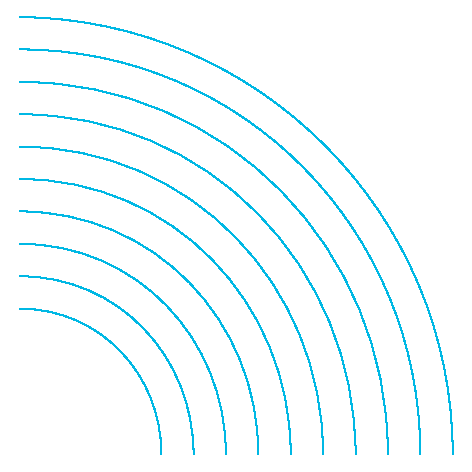
\includegraphics[width=.15\paperwidth,height=.15\paperwidth]{EETtemplateFiles/img/Simbolo_ESCOLA.pdf}\\
  
\includegraphics[width=.15\paperwidth,trim={.4cm .5cm .4cm 2.25cm},clip]{EETtemplateFiles/img/Logotipo_ESCOLA.pdf}
  \vspace*{-11pt}%
}

% MATH SYMBOLS

\newcommand{\field}[1]{\mathbb{#1}}

\DeclareMathOperator{\atan}{atan}
\DeclareMathOperator{\acos}{acos}
\DeclareMathOperator{\asin}{asin}

% \newcommand{\mb}[1]{\mathbf{#1}}


\newcommand{\A}{\mathbf{A}}
\newcommand{\B}{\mathbf{B}}
\newcommand{\Cb}{\mathbf{C}}
\newcommand{\D}{\mathbf{D}}
\newcommand{\Eb}{\mathbf{E}}
\newcommand{\F}{\mathbf{F}}
\newcommand{\Gb}{\mathbf{G}}
\newcommand{\Hb}{\mathbf{H}}
\newcommand{\I}{\mathbf{I}}
\newcommand{\J}{\mathbf{J}}
\newcommand{\Kb}{\mathbf{K}}
\newcommand{\Lb}{\mathbf{L}}
\newcommand{\M}{\mathbf{M}}
\newcommand{\N}{\mathbf{N}}
\newcommand{\Ob}{\mathbf{O}}
\newcommand{\Pb}{\mathbf{P}}
\newcommand{\Q}{\mathbf{Q}}
\newcommand{\R}{\mathbf{R}}
\newcommand{\Sb}{\mathbf{S}}
\newcommand{\T}{\mathbf{T}}
\newcommand{\U}{\mathbf{U}}
\newcommand{\V}{\mathbf{V}}
\newcommand{\W}{\mathbf{W}}
\newcommand{\X}{\mathbf{X}}
\newcommand{\Y}{\mathbf{Y}}
\newcommand{\Z}{\mathbf{Z}}
\newcommand{\Dl}{\mathbf{\boldsymbol{\Delta}}}
\newcommand{\Sg}{\mathbf{\boldsymbol{\Sigma}}}
\newcommand{\Ld}{\mathbf{\boldsymbol{\Lambda}}}
\newcommand{\Ph}{\mathbf{\boldsymbol{\Phi}}}
\newcommand{\Ps}{\mathbf{\boldsymbol{\Psi}}}
\newcommand{\Up}{\mathbf{\boldsymbol{\Upsilon}}}
\newcommand{\Xib}{\mathbf{\boldsymbol{\Xi}}}
% \newcommand{\D}{\mathbf{D}}
\newcommand{\one}{\mathbf{1}}
\newcommand{\zero}{\mathbf{0}}

\newcommand{\ab}{\mathbf{a}}
\newcommand{\bb}{\mathbf{b}}
\newcommand{\cc}{\mathbf{c}}
\newcommand{\dd}{\mathbf{d}}
\newcommand{\e}{\mathbf{e}}
\newcommand{\f}{\mathbf{f}}
\newcommand{\g}{\mathbf{g}}
\newcommand{\h}{\mathbf{h}}
\newcommand{\ib}{\mathbf{i}}
\newcommand{\jb}{\mathbf{j}}
\newcommand{\kb}{\mathbf{k}}
\newcommand{\lb}{\mathbf{\ell}}
\newcommand{\m}{\mathbf{m}}
\newcommand{\n}{\mathbf{n}}
\newcommand{\ob}{\mathbf{o}}
\newcommand{\pp}{\mathbf{p}}
\newcommand{\q}{\mathbf{q}}
\newcommand{\rr}{\mathbf{r}}
\newcommand{\s}{\mathbf{s}}
\newcommand{\uu}{\mathbf{u}}
\newcommand{\vv}{\mathbf{v}}
\newcommand{\w}{\mathbf{w}}
\newcommand{\x}{\mathbf{x}}
\newcommand{\y}{\mathbf{y}}
\newcommand{\z}{\mathbf{z}}
\newcommand{\al}{\mathbf{\boldsymbol{\alpha}}}
\newcommand{\vmu}{\mathbf{\boldsymbol{\mu}}}
\newcommand{\vlambda}{\mathbf{\boldsymbol{\lambda}}}
\newcommand{\vphi}{\mathbf{\boldsymbol{\phi}}}
\newcommand{\vpsi}{\mathbf{\boldsymbol{\psi}}}
\newcommand{\vrho}{\mathbf{\boldsymbol{\rho}}}
\newcommand{\vups}{\mathbf{\boldsymbol{\upsilon}}}
\newcommand{\vxi}{\mathbf{\boldsymbol{\xi}}}

\newcommand{\rank}{\textnormal{rank}}
% \newcommand{\trace}{\textnormal{trace}}
\newcommand{\exptr}{\textnormal{exptr}}
\newcommand{\tr}{\textnormal{tr}}
% \newcommand{\vstack}{\textnormal{vec}}
% \newcommand{\diag}{\textnormal{diag}}
\newcommand{\vstack}[1]{\Xib_{#1}}
\newcommand{\diag}[1]{\Ld_{#1}}
\newcommand{\tnsr}[2]{\underline{\mathsf{#1}}_{#2}}
\newcommand{\tmult}[1]{\underset{#1}{\times}}

\DeclareMathOperator{\Prob}{Prob}
%  |x>
\newcommand{\ket}[1]{\left\vert#1\right\rangle}
%  <x|
\newcommand{\bra}[1]{\left\langle#1\right\vert}
%  <x|y>
\newcommand{\braket}[2]{\left< #1 \vphantom{#2}\,
                        \right\vert\left.\!\vphantom{#1} #2 \right>}
%  <x|a|y>
\newcommand{\sandwich}[3]{\left< #1 \vphantom{#2 #3} \right|
                          #2 \min\left(\vphantom{#1 #2} #3 \right>}

\newcommand{\pd}[2]{\frac{\partial #1}{\partial #2}}
%  d/dt
\newcommand{\ddt}{\frac{d}{dt}}
%  D/Dx
\newcommand{\pdd}[1]{\frac{\partial}{\partial#1}}
%  |x|
\newcommand{\abs}[1]{\left\vert#1\right\vert}
%  k_{x}
\newcommand{\kv}[1]{\mathbf{k}_{#1}}
%  \textnormal{E}_{domain of integration}{variable}
\newcommand{\Ex}[2]{{\mathbb{E}_{#1}\left[#2\right]}}
\newcommand{\CEx}[3]{{\mathbb{E}_{#1}\left[#2|#3\right]}}
\newcommand{\CInf}[3]{{\textnormal{I}\left(#1;#2|#3\right)}}
\newcommand{\Inf}[2]{{\textnormal{I}\left(#1;#2\right)}}
\newcommand{\CEnt}[2]{{\textnormal{H}\left(#1|#2\right)}}
\newcommand{\Ent}[1]{{\textnormal{H}\left(#1\right)}}
\newcommand{\dCEnt}[2]{{\textnormal{h}\left(#1|#2\right)}}
\newcommand{\dEnt}[1]{{\textnormal{h}\left(#1\right)}}

\newcommand{\cmark}{\ding{51}}%
\newcommand{\xmark}{\ding{55}}%
\newcommand{\itempro}{\item[\textcolor{KYJade}{\Large \cmark}]}
\newcommand{\itemcontra}{\item[\textcolor{ARust}{\Large \xmark}]}
\newcommand\Tau{\mathcal{T}}
%Figure and format fixes


\renewcommand{\figurename}{Fig.}
\newcommand{\PESrule}{\noindent\rule{.57\columnwidth}{0.1mm}}

%theroem environments
% If using amsthm package, we need to delete these theorems before giving them our own definition. does not work for theorem
% \let\theorem\relax
\let\definition\relax
\let\lemma\relax
\let\corollary\relax
\let\example\relax
%
% \newtheorem{theorem}{Theorem}
\newtheorem{definition}{Definition}
\newtheorem{lemma}{Lemma}
\newtheorem{corollary}{Corollary}
\newtheorem{conjecture}{Conjecture}
\theoremstyle{plain}
\newtheorem{remark}{Remark}
\newtheorem{proposition}{Proposition}
\newtheorem{example}{Example}
\newtheorem{homework}{Homework}

%Colors
   \definecolor{blueH3}{rgb}{0,.5,1}
   \definecolor{blueH2}{rgb}{0,0.25,0.75}
   \definecolor{blueH1}{rgb}{0,0,0.5}   
   \definecolor{grayOldText}{rgb}{.5,.5,.5}
   \definecolor{VCobalt}{HTML}{005682}
   \definecolor{TZTeal}{HTML}{008080}
   \definecolor{TZTealfaded}{HTML}{F0FFFF}
   \definecolor{KYJade}{HTML}{008151}
   \definecolor{ARust}{HTML}{a10000}
   \definecolor{FFucsia}{HTML}{7000c3}   
   \definecolor{TAMustard}{HTML}{a1a100}
   \definecolor{Tangerine}{HTML}{d45500}
   
   
% Tikz 
% signal block diagram components
\tikzset{
    block/.style = {draw, rectangle, 
        minimum height=1cm, 
        minimum width=1.2cm, align=center},
    input/.style = {coordinate,node distance=1cm},
    output/.style = {coordinate,node distance=2cm},
    arrow/.style={draw, -latex,node distance=1.5cm},
    pinstyle/.style = {pin edge={latex-, black,node distance=1.5cm}},
    sum/.style = {draw, circle, node distance=1cm}
}
\tikzstyle{pinstyle} = [pin edge={to-,thin,black}]
\def\antenna{%
    -- +(0mm,4.0mm) -- +(2.625mm,7.5mm) -- +(-2.625mm,7.5mm) -- +(0mm,4.0mm) -- +(0mm,0mm)
}
% Overlay highlights on top of the page
\newcommand{\markOverlay}[1]{\tikz[overlay,remember picture] \node (#1) {};}
\newcommand{\drawOverlayBox}[4][]{%
    \tikz[overlay,remember picture]{%
        \coordinate (TopLeft)     at ($(#2)+(-0.4em,1.6em)$);
        \coordinate (BottomRight) at ($(#3)+(0.4em,-1.0em)$);
        %
        \path (TopLeft); \pgfgetlastxy{\XCoord}{\IgnoreCoord};
        \path (BottomRight); \pgfgetlastxy{\IgnoreCoord}{\YCoord};
        \coordinate (LabelPoint) at ($(\XCoord,\YCoord)!0.5!(BottomRight)$);
        %
        \draw [red,#1] (TopLeft) rectangle (BottomRight);
        \node [below, #1, fill=none, fill opacity=1] at (LabelPoint) {#4};
    }
}
\newcommand{\drawOverlayLine}[4][]{%
    \tikz[overlay,remember picture]{%
        \draw [red,#1] ($(#2)$) -- node{#4} ($(#3)$);
    }
}
\newcommand{\drawOverlayCircle}[4][]{%
    \tikz[overlay,remember picture]{%
        \draw [red,#1] ($(#2)$) circle (#3) node{#4};
    }
}
   
   %%%%%%%%%%%%%%%%%%%%%%%%%%%%%%%%%%%%%%%%%%%%%%%%%%%%%%%%%%%%%%%%%
%% The following definitions are to extend the LaTeX algorithmic 
%% package with SWITCH statements and one-line structures.
%% The extension is by 
%%   Prof. Farn Wang 
%%   Dept. of Electrical Engineering, 
%%   National Taiwan University. 
%% 
\newcommand{\SWITCH}[1]{\STATE \textbf{switch} (#1)}
\newcommand{\ENDSWITCH}{\STATE \textbf{end switch}}
\newcommand{\CASE}[1]{\STATE \textbf{case} #1\textbf{:} \begin{ALC@g}}
\newcommand{\ENDCASE}{\end{ALC@g}}
\newcommand{\CASELINE}[1]{\STATE \textbf{case} #1\textbf{:} }
\newcommand{\DEFAULT}{\STATE \textbf{default:} \begin{ALC@g}}
\newcommand{\ENDDEFAULT}{\end{ALC@g}}
\newcommand{\DEFAULTLINE}[1]{\STATE \textbf{default:} }
%% 
%% End of the LaTeX algorithmic package extension.

\newcounter{MYtempeqncnt}


%%%%%%%%%%%%%%%%%%%%%%%%%%%%%%%%%%%%%%%
% Commands to recall text later
%%%%%%%%%%%%%%%%%%%%%%%%%%%%%%%%%%%%%%%
\makeatletter
\newcommand\remembertext[2]{% #1 is a key, #2 is the text
  \immediate\write\@auxout{\unexpanded{\global\long\@namedef{mytext@#1}{#2}}}%
  #2%
}
%
\newcommand\recalltext[1]{%
  \ifcsname mytext@#1\endcsname
    \@nameuse{mytext@#1}%
  \else
    ``??''
  \fi
}

%%%%%%%%%%%%%%%%%%%%%%%%%%%%%%%%%%%%%%%%%%%%%%%%%%%%%%%%%%%%%%%%%%%%%%%%%%%%%%%%%%
%%% Paolo Casari: macros for automating section titling and comment formatting %%%
%%%%%%%%%%%%%%%%%%%%%%%%%%%%%%%%%%%%%%%%%%%%%%%%%%%%%%%%%%%%%%%%%%%%%%%%%%%%%%%%%%
\newcounter{myequationcnt}

\newcounter{rcnt}
\newcounter{ccnt}

\newcommand{\newreviewernopagebreak}[1]{\vspace{5em} \setcounter{ccnt}{0}\section*{\normalsize Comments of #1}\vspace{4mm}}

\newcommand{\ThisIsTheEditorNoPageBreak}{\setcounter{ccnt}{0}\section*{\Large Comments of the Editor}\vspace{3mm}}
\newcommand{\ThisIsTheEditor}{\clearpage \ThisIsTheEditorNoPageBreak}
\newcommand{\ThisIsANewReviewerNoPageBreak}[1]{\vspace{5em} \refstepcounter{rcnt}\label{r#1}\setcounter{ccnt}{0}\section*{\Large Comments of Reviewer \arabic{rcnt}}\vspace{3mm}}
\newcommand{\ThisIsANewReviewer}[1]{\clearpage\vspace{-5em} \ThisIsANewReviewerNoPageBreak{#1}}

\newcommand{\edcomment}[1]{
\begin{tcbremark}
\color{VCobalt}
    \refstepcounter{ccnt}\label{e\arabic{ccnt}}\noindent\textbf{\boldmath\emph{Comment E.\arabic{ccnt}:}} #1\vspace{0.2cm}
\end{tcbremark}
}
\newcommand{\refedcomment}[1]{E.\ref{e#1}}

\newcommand{\revcomment}[1]{
\begin{tcbremark}
\color{VCobalt}
\refstepcounter{ccnt}\label{r\arabic{rcnt}c\arabic{ccnt}}\noindent\textbf{\boldmath\emph{Comment \arabic{rcnt}.\arabic{ccnt}:}} #1\vspace{0.2cm}
\end{tcbremark}
}
\newcommand{\refrevcomment}[2]{\ref{r#1}.\ref{r#1c#2}}

% \newcommand{\ouranswer}[1]{\noindent\emph{Answer:} #1\vspace{0.6cm}}
% \newcommand{\citepap}[1]{\vspace{0.33cm}\begin{minipage}{0.05\textwidth} $\phantom{A}$  \end{minipage}\begin{minipage}{0.85\textwidth}\renewcommand{\baselinestretch}{1.15}\small \emph{#1} \end{minipage}\vspace{0.3cm}}

\newlength{\ansspace}
\addtolength{\ansspace}{0.6cm}
\newcommand{\ansbreak}{\vspace{\ansspace}}

\newlength{\stdleftskip}
\addtolength{\stdleftskip}{\leftskip}
\newlength{\stdrightskip}
\addtolength{\stdrightskip}{\rightskip}
\newlength{\citeskip}
\addtolength{\citeskip}{2em}
\newcommand{\oldbaselinestretch}{1.5}

\newcommand{\setcitepapskip}{%
    \leftskip\citeskip %
    \rightskip\citeskip %
    \renewcommand{\baselinestretch}{1.15}\small%
    \vspace{0.6em}%
    \noindent%
}

\newcommand{\resetLRmargins}{%
    \leftskip\stdleftskip %
    \rightskip\stdrightskip %
    \renewcommand{\baselinestretch}{\oldbaselinestretch}\normalsize %
    \vspace{0.6em}
}

\newcommand{\emans}{\emph{Answer:\ }}


%---------------
% LIMIAR
%---------------
%configuracion de opcions de beamer persoais, pero alleas ao estilo

% COMANDO QUE INTRODUCE UNHA DIAPOSITIVA CUN ÍNDICE NO QUE APARECEN VELADAS TÓDALAS SECCIÓNS MENOS A ACTUAL. ÚTIL PARA INTRODUCIR OS TÍPICOS ÍNDICES INTERMEDIOS.
\newcommand{\Inter}{\frame{\tableofcontents[currentsection]}}
\newcommand{\inter}{\frame{\tableofcontents[currentsection,currentsubsection]}}

% Pes de imaxe
\renewcommand{\figurename}{Fig.}
\addto\captionsenglish{\renewcommand{\figurename}{Fig.}}
\setbeamertemplate{caption}[numbered]

%ESTE PAQUETE PERMITE POÑER A BIBLIOGRAFIA AO PE DE PAXINA CON CONFIGURACIONS ESTETICAS PERSOAIS
% \usepackage[style=ieee,doi=false,isbn=false,url=true,backend=bibtex]{biblatex}
% \bibliography{./bibliografia.bib}
% \newrobustcmd*{\footfullcitenomark}{%
%   \AtNextCite{%
%     \let\thefootnote\relax 
%     \let\mkbibfootnote\mkbibfootnotetext
%     }%
%   \footfullcite}

%paquete para engadir notas de guion ao pdf
\usepackage{pgfpages}
% \setbeameroption{show only notes} 
% \setbeameroption{show notes}
% \setbeameroption{show notes on second screen=right}
% DATOS DO DOCUMENTO
\title[CDA]{Advanced Digital Communications}
\subtitle{Session 5: Diversity, STC and Limited CSIT}
\author[FGC]{\underline{Felipe G\'omez-Cuba}}
\institute[GPSC]{
\begin{columns}[T]
\begin{column}{5cm}\centering
Office A-204\\
Wednesday \& Thursday 15:00-18:00\\
\texttt{gomezcuba@gts.uvigo.es}\\
\end{column}
\end{columns}
}

\date{2025}

\begin{document}

% Diapositiva co título
\frame[plain]{\titlepage}

\frame{\frametitle{SIMO Channel}
\begin{columns}
 \begin{column}{6cm}    
    \begin{figure}
    \centering
%     \caption{Maximum Ratio Combining}
    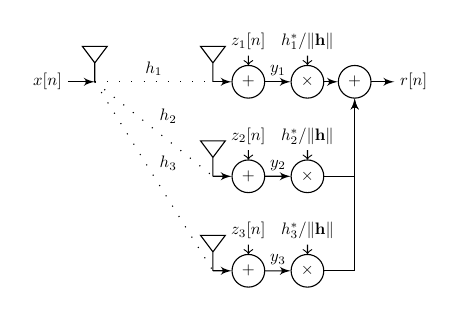
\begin{tikzpicture}[auto, node distance=2cm,>=latex', scale=0.6, every node/.style={scale=0.6}]
        \node [pinstyle, name=input] {$x[n]$};
        \node [input, right of=input, node distance=1cm, name=txant] {};
        \draw [draw] (txant) \antenna;
        \draw [draw,->,align=center] (input) -- (txant);
        \node [input, right of=txant, node distance=2.5cm, name=rxant1] {};
        \draw [draw,loosely dotted,-,align=center] (txant)  -- node {$h_1$} (rxant1);
        \foreach \a [evaluate=\a as \prev using int(\a-1)] in {2,3}{
            \node [input, below of=rxant\prev, node distance=2cm, name=rxant\a] {}; 
            \draw [draw,loosely dotted,-,align=center] (txant)  -- node {$h_\a$} (rxant\a);
            }
        \foreach \a in {1,2,...,3}{
            \draw [draw] (rxant\a) \antenna;
            \node [sum, right of=rxant\a, node distance=.75cm, pin={[pinstyle,pin distance=.2cm]above:$z_\a[n]$}] (sum\a) {$+$};
            \draw [draw,->,align=center] (rxant\a) -- (sum\a);
            \node [sum,right of=sum\a, node distance=1.25cm, pin={[pinstyle, pin distance=.2cm]above:$h_\a^*/\|\h\|$}] (mult\a) {$\times$};
            \draw [draw,->,align=center] (sum\a) -- node {$y_\a$} (mult\a);
%             \noce [block, right of=sum\a, node distance=1cm] (weight\a) {$w_\a$};
%             \draw [draw,->,align=center] (sum\a) -- (weight\a);
        }
        \node [sum, right of=mult1, name=sumacc] {$+$};
        \draw [draw,->,align=center] (mult1) -- (sumacc);
        \foreach \a in {2,3}{
            \draw [draw,->,align=center] (mult\a) -| (sumacc);
        }
        \node [pinstyle, right of=sumacc, node distance=1.25cm, name=output] {$r[n]$};
        \draw[->] (sumacc) -- (output);
        \end{tikzpicture}
\end{figure}
%     $$\rho=\frac{P\sum_{i=1}^{N_{r}}|h_i|^2}{\sigma_z^2}\sim \frac{P}{\sigma_z^2\sqrt{2}}\chi^2(2N_{r})$$
% \begin{itemize}
%  \item Array Gain $\overline{\rho}=N_{r}\frac{P}{\sigma_z^2}$
%  \item Diversity $P_o\propto \overline{\rho}^{-N_{r}}$
%  \end{itemize}
 \end{column}
 \begin{column}{6cm}    
    \begin{figure}
    \centering
%     \caption{Selection Combining}
    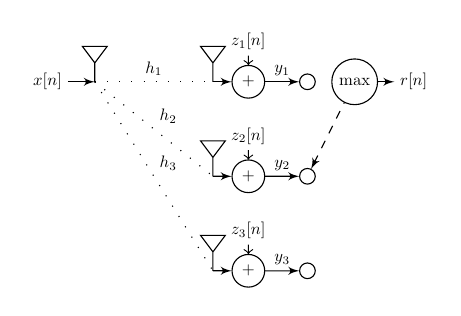
\begin{tikzpicture}[auto, node distance=2cm,>=latex', scale=0.6, every node/.style={scale=0.6}]
        \node [pinstyle, name=input] {$x[n]$};
        \node [input, right of=input, node distance=1cm, name=txant] {};
        \draw [draw] (txant) \antenna;
        \draw [draw,->,align=center] (input) -- (txant);
        \node [input, right of=txant, node distance=2.5cm, name=rxant1] {};
        \draw [draw,loosely dotted,-,align=center] (txant)  -- node {$h_1$} (rxant1);
        \foreach \a [evaluate=\a as \prev using int(\a-1)] in {2,3}{
            \node [input, below of=rxant\prev, node distance=2cm, name=rxant\a] {}; 
            \draw [draw,loosely dotted,-,align=center] (txant)  -- node {$h_\a$} (rxant\a);
            }
        \foreach \a in {1,2,...,3}{
            \draw [draw] (rxant\a) \antenna;
            \node [sum, right of=rxant\a, node distance=.75cm, pin={[pinstyle,pin distance=.2cm]above:$z_\a[n]$}] (sum\a) {$+$};
            \draw [draw,->,align=center] (rxant\a) -- (sum\a);
            \node [sum,right of=sum\a, node distance=1.25cm] (mult\a) {};
            \draw [draw,->,align=center] (sum\a) -- node {$y_\a$} (mult\a);
%             \noce [block, right of=sum\a, node distance=1cm] (weight\a) {$w_\a$};
%             \draw [draw,->,align=center] (sum\a) -- (weight\a);
        }
        \node [sum, right of=mult1, name=sumacc] {$\max$};
        \draw [draw,<-,dashed,align=center] (mult2) -- (sumacc);
%         \foreach \a in {2,3}{
%             \draw [draw,->,align=center] (mult\a) -| (sumacc);
%         }
        \node [pinstyle, right of=sumacc, node distance=1.25cm, name=output] {$r[n]$};
        \draw[->] (sumacc) -- (output);
        \end{tikzpicture}
\end{figure}
%     $$\rho=\frac{ P\max_{\{1\dots N_{r}\}} |h_i|^2}{\sigma_z^2}\sim \textnormal{MaxExp}(N_{r},\frac{\sigma_z^2}{P})$$
% \begin{itemize}
%  \item $\overline{\rho}=\left(\sum_{k=1}^{N_{r}}{N_{r} \choose k}\frac{(1)^{k-1}}{k}\right)\frac{P}{\sigma_z^2}$
%  \item Diversity $P_o\propto \overline{\rho}^{-N_{r}}$
%  \end{itemize}
 \end{column}
\end{columns}
\begin{table}
  \begin{tabular}{c|c|c}
   &Maximal Ratio Combining& Selection Combining\\\hline
   $\rho=$&$\frac{P\sum_{i=1}^{N_{r}}|h_i|^2}{\sigma_z^2}$& $\rho=\frac{ P\max_{\{1\dots N_{r}\}} |h_i|^2}{\sigma_z^2}$\\
   $f(\frac{\rho}{P/\sigma_z^2})\sim$&$\frac{1}{\sqrt{2}}\chi^2(2N_{r})$& $\max\textnormal{-}N_{r}\textnormal{-}\textnormal{Exp}(1)$\\
   Array Gain&$\overline{\rho}=N_{r}\frac{P}{\sigma_z^2}$& $\overline{\rho}=\left(\sum_{k=1}^{N_{r}}{N_{r} \choose k}\frac{(1)^{k-1}}{k}\right)\frac{P}{\sigma_z^2}$\\\hline
   Diversity& \multicolumn{2}{c}{$P_o\approx\overline{\rho}^{-N_{r}}$}
  \end{tabular}
\end{table}
}

\frame{\frametitle{MISO Channel with CSIT}

\begin{columns}
 \begin{column}{6cm}    
    \begin{figure}
    \centering
%     \caption{Maximum Ratio Combining}
    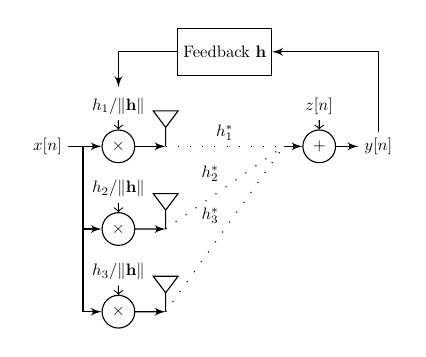
\begin{tikzpicture}[auto, node distance=2cm,>=latex', scale=0.6, every node/.style={scale=0.6}]
        \node [pinstyle, name=input1] {$x[n]$};
        \node [coordinate,right of=input1,node distance=.75cm, name=split] {};
        \draw [draw,-,align=center] (input1) -- (split);
            \node [sum,right of=split, node distance=.75cm, pin={[pinstyle, pin distance=.2cm]above:$h_1/\|\h\|$}] (mult1) {$\times$};
            \draw [draw,->,align=center] (split) -- (mult1);        
        \foreach \a [evaluate=\a as \prev using int(\a-1)] in {2,3}{
            \node [sum,below of=mult\prev, node distance=1.75cm, pin={[pinstyle, pin distance=.2cm]above:$h_\a/\|\h\|$}] (mult\a) {$\times$};
            \draw [draw,->,align=center] (split) |- (mult\a);
        }
        \foreach \a in {1,2,...,3}{
            \node [input, right of=mult\a, node distance=1cm, name=txant\a] {};
            \draw [draw] (txant\a) \antenna;
            \draw [draw,->,align=center] (mult\a) -- (txant\a);
            }
        \node [input, right of=txant1, node distance=2.5cm, name=rxant1] {};
        \foreach \a [evaluate=\a as \prev using int(\a-1)] in {1,2,3}{
            \draw [draw,loosely dotted,-,align=center] (txant\a)  -- node {$h_\a^*$} (rxant1);
            }
%             \draw [draw] (rxant1) \antenna;
    \node [sum, right of=rxant1, node distance=.75cm, pin={[pinstyle, pin distance=.2cm]above:$z[n]$}] (sumacc) {$+$};
    \draw [draw,->,align=center] (rxant1) -- (sumacc);
    \node [pinstyle, right of=sumacc, node distance=1.25cm, name=output] {$y[n]$};  
    \draw[->] (sumacc) -- (output);
    \node[block] (fb) at ($(txant1)!.5!(rxant1)+(0,2)$) {Feedback $\h$};
    \draw[->] (output) |- (fb);
    \draw[->] (fb) -| ($(mult1)+(0,1.25)$);
        \end{tikzpicture}
\end{figure}
%     $$\rho=\frac{P\sum_{i=1}^{N_{r}}|h_i|^2}{\sigma_z^2}\sim \frac{P}{\sigma_z^2\sqrt{2}}\chi^2(2N_{r})$$
% \begin{itemize}
%  \item Array Gain $\overline{\rho}=N_{r}\frac{P}{\sigma_z^2}$
%  \item Diversity $P_o\propto \overline{\rho}^{-N_{r}}$
%  \end{itemize}
 \end{column}
 \begin{column}{6cm} 
    \begin{figure}
    \centering
%     \caption{Maximum Ratio Combining}
    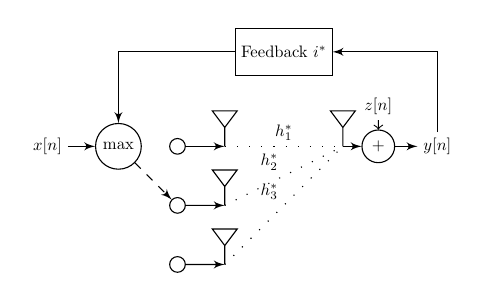
\begin{tikzpicture}[auto, node distance=2cm,>=latex', scale=0.6, every node/.style={scale=0.6}]
        \node [pinstyle, name=input1] {$x[n]$};
        \node [sum, right of=input1, name=split, node distance=1.5cm] {$\max$};
        \draw [draw,->,align=center] (input1) -- (split);        
            \node [sum,right of=split, node distance=1.25cm] (mult1) {};
        \foreach \a [evaluate=\a as \prev using int(\a-1)] in {2,3}{
            \node [sum,below of=mult\prev, node distance=1.25cm] (mult\a) {};  
        }
        \draw [draw,->,dashed,align=center] (split) -- (mult2);
        \foreach \a in {1,2,...,3}{
            \node [input, right of=mult\a, node distance=1cm, name=txant\a] {};
            \draw [draw] (txant\a) \antenna;
            \draw [draw,->,align=center] (mult\a) -- (txant\a);
            }
        \node [input, right of=txant1, node distance=2.5cm, name=rxant1] {};
        \foreach \a [evaluate=\a as \prev using int(\a-1)] in {1,2,3}{
            \draw [draw,loosely dotted,-,align=center] (txant\a)  -- node {$h_\a^*$} (rxant1);
            }
            \draw [draw] (rxant1) \antenna;
    \node [sum, right of=rxant1, node distance=.75cm, pin={[pinstyle, pin distance=.2cm]above:$z[n]$}] (sumacc) {$+$};
    \draw [draw,->,align=center] (rxant1) -- (sumacc);
    \node [pinstyle, right of=sumacc, node distance=1.25cm, name=output] {$y[n]$};
    \draw[->] (sumacc) -- (output);
    \node[block] (fb) at ($(txant1)!.5!(rxant1)+(0,2)$) {Feedback $i^*$};
    \draw[->] (output) |- (fb);
    \draw[->] (fb) -| (split);
        \end{tikzpicture}
%   
\end{figure}
% %     $$\rho=\frac{ P\max_{\{1\dots N_{r}\}} |h_i|^2}{\sigma_z^2}\sim \textnormal{MaxExp}(N_{r},\frac{\sigma_z^2}{P})$$
% % \begin{itemize}
% %  \item $\overline{\rho}=\left(\sum_{k=1}^{N_{r}}{N_{r} \choose k}\frac{(1)^{k-1}}{k}\right)\frac{P}{\sigma_z^2}$
% %  \item Diversity $P_o\propto \overline{\rho}^{-N_{r}}$
% %  \end{itemize}
 \end{column}
\end{columns}
\begin{table}
  \begin{tabular}{c|c|c}
   &Maximal Ratio Combining& Selection Combining\\\hline
   Required CSIT & $\h$ ($2N_{t}\times$ \texttt{\color{KYJade}float}) & $i^*$ ($1\times$ \texttt{\color{KYJade} int})\\
   $\rho=$&$\frac{P\sum_{i=1}^{N_{t}}|h_i|^2}{\sigma_z^2}$& $\rho=\frac{ P\max_{\{1\dots N_{t}\}} |h_i|^2}{\sigma_z^2}$\\
   $f(\frac{\rho}{P/\sigma_z^2})\sim$&$\frac{1}{\sqrt{2}}\chi^2(2N_{t})$& $\max\textnormal{-}N_{t}\textnormal{-}\textnormal{Exp}(1)$\\
   Array Gain&$\overline{\rho}=N_{t}\frac{P}{\sigma_z^2}$& $\overline{\rho}=\left(\sum_{k=1}^{N_{t}}{N_{t} \choose k}\frac{(1)^{k-1}}{k}\right)\frac{P}{\sigma_z^2}$\\\hline
   Diversity& \multicolumn{2}{c}{$P_o\approx\overline{\rho}^{-N_{t}}$}
  \end{tabular}
\end{table}
}

\frame{\frametitle{MISO Channel without CSIT}

\begin{columns}
 \begin{column}{6cm}    
    \begin{figure}
    \centering
    \caption{Uncoded MISO with No-CSIT }
    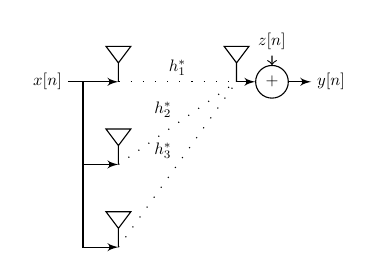
\begin{tikzpicture}[auto, node distance=2cm,>=latex', scale=0.6, every node/.style={scale=0.6}]
        \node [pinstyle, name=input1] {$x[n]$};
        \node [coordinate,right of=input1,node distance=.75cm, name=split] {};
        \draw [draw,-,align=center] (input1) -- (split);
        \node [input,right of=split, node distance=.75cm, name=txant1] {};
            \draw [draw] (txant1) \antenna;
            \draw [draw,->,align=center] (split) -- (txant1);        
        \foreach \a [evaluate=\a as \prev using int(\a-1)] in {2,3}{
            \node [input,below of=txant\prev, node distance=1.75cm, name=txant\a] {};
            \draw [draw] (txant\a) \antenna;
            \draw [draw,->,align=center] (split) |- (txant\a);
            }
        \node [input, right of=txant1, node distance=2.5cm, name=rxant1] {};
        \foreach \a [evaluate=\a as \prev using int(\a-1)] in {1,2,3}{
            \draw [draw,loosely dotted,-,align=center] (txant\a)  -- node {$h_\a^*$} (rxant1);
            }
            \draw [draw] (rxant1) \antenna;
    \node [sum, right of=rxant1, node distance=.75cm, pin={[pinstyle, pin distance=.2cm]above:$z[n]$}] (sumacc) {$+$};
    \draw [draw,->,align=center] (rxant1) -- (sumacc);
    \node [pinstyle, right of=sumacc, node distance=1.25cm, name=output] {$y[n]$};  
    \draw[->] (sumacc) -- (output);
        \end{tikzpicture}
\end{figure}
 \end{column}
 \begin{column}{6cm}
 
    $$\rho=\frac{P|\sum_{i=1}^{N_{t}}h_i|^2}{N_{t}\sigma_z^2}\sim \frac{P}{\sigma_z^2}Exp(1)$$
\begin{itemize}
 \item No Array Gain $\overline{\rho}=\frac{P}{\sigma_z^2}$
 \item No Diversity $P_o\propto \overline{\rho}^{-1}$
 \end{itemize}
 \end{column}
\end{columns}
}


\frame{\frametitle{MISO with Time Diversity}

\begin{columns}
 \begin{column}{5cm}    
    \begin{figure}
    \centering
    \caption{Delay Diversity Coding}
    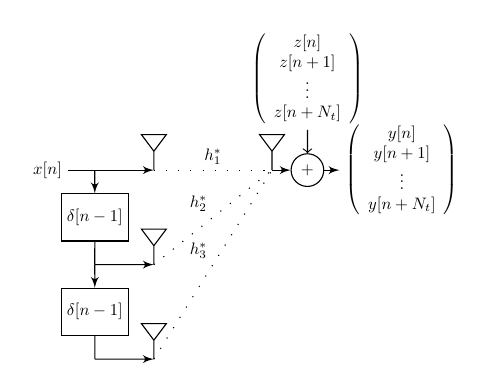
\begin{tikzpicture}[auto, node distance=2cm,>=latex', scale=0.6, every node/.style={scale=0.6}]
        \node [pinstyle, name=input1] {$x[n]$};
        \node [coordinate,right of=input1,node distance=.5cm, name=split] {};
        \draw [draw,-,align=center] (input1) -- (split);
        \node [coordinate,right of=split, node distance=.5cm] (mult1) {};
        \draw [draw,-,align=center] (split) -- (mult1);        
        \foreach \a [evaluate=\a as \prev using int(\a-1)] in {2,3}{
            \node [coordinate,below of=mult\prev, node distance=2cm] (mult\a) {};
            \node [block,below of=mult\prev, node distance=1cm] (del\prev) {$\delta[n-1]$};
            \draw [draw,->,align=center] (mult\prev) -- (del\prev);
            \draw [draw,-,align=center] (del\prev) -- (mult\a);
        }
        \foreach \a in {1,2,...,3}{
            \node [input, right of=mult\a, node distance=1.25cm, name=txant\a] {};
            \draw [draw] (txant\a) \antenna;
            \draw [draw,->,align=center] (mult\a) -- (txant\a);
            }
        \node [input, right of=txant1, node distance=2.5cm, name=rxant1] {};
        \foreach \a [evaluate=\a as \prev using int(\a-1)] in {1,2,3}{
            \draw [draw,loosely dotted,-,align=center] (txant\a)  -- node {$h_\a^*$} (rxant1);
            }
            \draw [draw] (rxant1) \antenna;
    \node [sum, right of=rxant1, node distance=.75cm, pin={[pinstyle, pin distance=.5cm]above:$\left(\begin{array}{c}z[n]\\z[n+1]\\\vdots\\z[n+N_{t}]\end{array}\right)$}] (sumacc) {$+$};
    \draw [draw,->,align=center] (rxant1) -- (sumacc);
    \node [pinstyle, right of=sumacc, node distance=2cm, name=output] {$\left(\begin{array}{c}y[n]\\y[n+1]\\\vdots\\y[n+N_{t}]\end{array}\right)$};  
    \draw[->] (sumacc) -- (output);
        \end{tikzpicture}
\end{figure}
  \begin{itemize}
   \item Virtual Time Diversity in Slow Fading!
  \end{itemize}
 \end{column}
 \begin{column}{7cm}
  \begin{itemize}
   \item Virtual SIMO equivalent
   $$\y
%    =\left(\begin{array}{c}y[n]\\y[n+1]\\\vdots\\y[n+N_{t}]\end{array}\right)
%    =\left(\begin{array}{c}h_1\\h_2\\\vdots\\h_{N_{t}}\end{array}\right)x[n]+\left(\begin{array}{c}z[n]\\z[n+1]\\\vdots\\z[n+N_{t}]\end{array}\right)
=\h x[n]+\z $$
   \item MRC/Selection Diversity $P_o\approx \overline{\rho}^{-N_{t}}$\\ \ \\
   \item Array Gain $\overline{\rho}=\frac{N_{t}P}{\sigma_z^2}$\\ \ \\
   \item Space-Time Code rate $\frac{1}{N_{t}}$
   $$\Gb_{x[n]}=\left(\begin{array}{cccc}
            x[n]&0&0\\
            0&x[n]&0\\
            \vdots&\vdots&\ddots&\vdots\\
            0&0&\dots&x[n]\\
\end{array}\right)=\I_{N_{t}}x[n]$$
   $$\y=\Gb_{x[n]}\h+\z$$
  \end{itemize}
 \end{column}
\end{columns}
}


\frame{\frametitle{MISO with Alamouti}

\begin{columns}
 \begin{column}{6cm}    
    \begin{figure}
    \centering
    \caption{Alamoutti Scheme}
    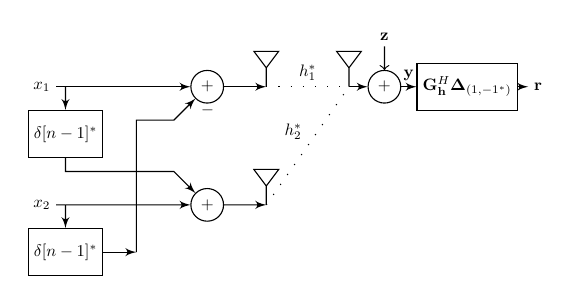
\begin{tikzpicture}[auto, node distance=2cm,>=latex', scale=0.6, every node/.style={scale=0.6}]
        \node [pinstyle, name=input1] {$x_1$};
        \node [pinstyle,below of=input1, node distance=2.5cm, name=input2] {$x_2$};        
        \node [coordinate,right of=input1,node distance=.5cm, name=split1] {};        
        \node [coordinate,right of=input2,node distance=.5cm, name=split2] {};
        \draw [draw,-,align=center] (input1) -- (split1);
        \draw [draw,-,align=center] (input2) -- (split2);
        \node [block,below of=split1, node distance=1cm] (del1) {$\delta[n-1]^*$};
        \node [block,below of=split2, node distance=1cm] (del2) {$\delta[n-1]^*$};
        \draw [draw,->,align=center] (split1) -- (del1);        
        \draw [draw,->,align=center] (split2) -- (del2);     
        \node [sum, right of=split1, node distance=3cm] (sum1) {$+$};   
        \node [sum, right of=split2, node distance=3cm] (sum2) {$+$};   
        \draw [draw,->,align=center] (split1) -- (sum1);        
        \draw [draw,->,align=center] (split2) -- (sum2);  
        \node[coordinate] (s2d) at($(sum2)+(135:1)$) {};
        \draw [->] (del1) |- (s2d) --  (sum2);
        \node [coordinate,right of=del2, node distance=1.5cm] (corner) {};
        \draw [->] (del2) -- (corner);
        \node[coordinate] (s1d) at($(sum1)+(225:1)$) {};
        \draw [->] (corner) |- (s1d) -- node[pos=0.99,anchor=north west] {$-$} (sum1);
        \foreach \a in {1,2}{
            \node [input, right of=sum\a, node distance=1.25cm, name=txant\a] {};
            \node [input, right of=txant1, node distance=1.75cm, name=rxant1] {};
            \draw [draw] (txant\a) \antenna;
            \draw [draw,->,align=center] (sum\a) -- (txant\a);
            \draw [draw,loosely dotted,-,align=center] (txant\a)  -- node {$h_\a^*$} (rxant1);
            }
            \draw [draw] (rxant1) \antenna;
    \node [sum, right of=rxant1, node distance=.75cm, pin={[pinstyle, pin distance=.5cm]above:$\z$}] (sumacc) {$+$};
    \draw [draw,->,align=center] (rxant1) -- (sumacc);
    \node [block, right of=sumacc, node distance=1.75cm, name=wf] {$\Gb_{\h}^H\Dl_{(1,-1^*)}$};  
    \node [pinstyle, right of=wf, node distance=1.5cm, name=output] {$\rr$};  
    \draw[->] (sumacc) -- node {$\y$} (wf);
    \draw[->] (wf) -- (output);
        \end{tikzpicture}
\end{figure}
  \begin{itemize}
   \item Space-Time Code \textbf{rate $1$}
   $$\Gb_{\x}=\left(\begin{array}{cc}
            x_1&-x_2^*\\
            x_2&x_1^*\\
\end{array}\right)$$
  \end{itemize}
 \end{column}
 \begin{column}{6cm}
  \begin{itemize}
   \item Virtual MIMO Equivalent
   $$\y=\Gb_{\x}\h+\z$$
   \item Negative Conjugate $y_2$
   $$\y'=\left(\begin{array}{cc}y_1\\-y_2^*\end{array}\right)=\Gb_{\h}\x+\z$$
   \item Unitary Virtual Channel (\textcolor{ARust}{ML!})
   $$\Gb_{\h}^H\Gb_{\h}=(|h_1|^2+|h_2|^2)\I_2$$
   \item Diversity $P_o\approx \overline{\rho}^{-2}$
   \item No Array Gain $\overline{\rho}=\frac{P}{\sigma_z^2}$
  \end{itemize}
 \end{column}
\end{columns}
}

\frame{\frametitle{General Space Time Coding}

\begin{columns}
 \begin{column}{6cm}    
    \begin{figure}
    \centering
    \caption{STC with bits}
    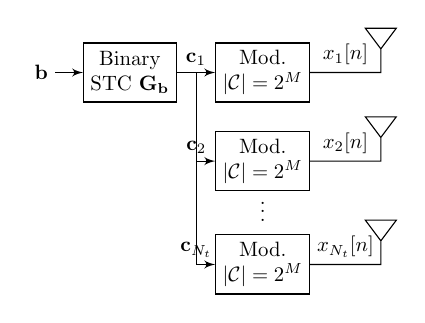
\begin{tikzpicture}[auto, node distance=1.5cm,>=latex', scale=0.75, every node/.style={scale=0.75}]
        \node [pinstyle] (input)  {$\bb$};
        \node [block, right of=input] (sp) {Binary\\STC $\Gb_{\bb}$};
        \draw[->] (input) -- (sp);
        \node [block, right of=sp, node distance=2.25cm] (mod1) {Mod.\\$|\mathcal{C}|=2^M$};
        \node [block, below of=mod1] (mod2) {Mod.\\$|\mathcal{C}|=2^M$};
        \node [below of=mod2, node distance=.75cm] (moddots) {$\vdots$};
        \node [block, below of=moddots, node distance=1cm] (modn) {Mod.\\$|\mathcal{C}|=2^M$};
        \draw[->] (sp) -- node{$\cc_1$} (mod1);
        \draw[->] (sp) -| ($(sp)!.5!(mod2)$) |- node{$\cc_2$}  (mod2);
        \draw[->] (sp) -| ($(sp)!.5!(mod2)$) |- node{$\cc_{N_{t}}$}  (modn);
        \node [output, right of=mod1, node distance=2cm] (ant1) {};
        \node [output, right of=mod2, node distance=2cm] (ant2) {};
        \node [output, right of=modn, node distance=2cm] (antn) {};
        \draw [-] (mod1) -- node {$x_1[n]$} (ant1) \antenna;            
        \draw [-] (mod2) -- node {$x_2[n]$} (ant2) \antenna;            
        \draw [-] (modn) -- node {$x_{N_{t}}[n]$} (antn) \antenna;    
    \end{tikzpicture}
\end{figure}
 \end{column}
 \begin{column}{6cm}    
    \begin{figure}
    \centering
    \caption{STC with Symbols}
    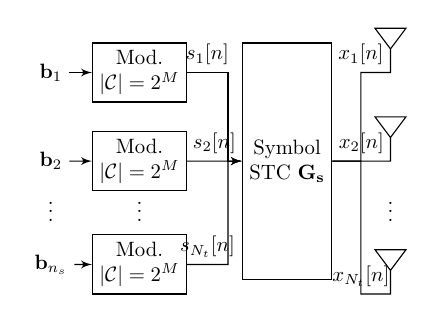
\begin{tikzpicture}[auto, node distance=1.5cm,>=latex', scale=0.75, every node/.style={scale=0.75}]
        \node [pinstyle] (input1)  {$\bb_1$};
        \node [pinstyle, below of=input1] (input2)  {$\bb_2$};
        \node [below of=input2, node distance=.75cm] (idots) {$\vdots$};
        \node [pinstyle, below of=idots, node distance=1cm] (inputn) {$\bb_{n_s}$};
        \node [block, right of=input1] (mod1)  {Mod.\\$|\mathcal{C}|=2^M$};
        \node [block, right of=input2] (mod2) {Mod.\\$|\mathcal{C}|=2^M$};
        \node [below of=mod2, node distance=.75cm] (moddots) {$\vdots$};
        \node [block, right of=inputn] (modn) {Mod.\\$|\mathcal{C}|=2^M$};
        \draw[->] (input1) --  (mod1);
        \draw[->] (input2) --  (mod2);
        \draw[->] (inputn) --  (modn);
        \node [block,right of=mod2,node distance=2.5cm,minimum height=4cm] (sstc) {Symbol\\
        STC $\Gb_{\s}$} ;
        \draw [->] (mod1) -- node{$s_1[n]$}  ($(mod1)+(1.5,0)$) |- (sstc);
        \draw [->] (mod2) -- node {$s_2[n]$} (sstc);
        \draw [->] (modn) -- node {$s_{N_{t}}[n]$} ($(modn)+(1.5,0)$) |- (sstc);
        \node [output, right of=sstc,node distance=1.75cm] (ant2) {};
        \node [output, above of=ant2, node distance=1.5cm] (ant1) {};
        \node [below of=ant2, node distance=.75cm] (antdots) {$\vdots$};
        \node [output, below of=antdots, node distance=1.5cm] (antn) {};
        \draw [-] (sstc) -- ($(sstc)+(1.25,0)$) |- node {$x_1[n]$} (ant1) \antenna;            
        \draw [-] (sstc) -- node {$x_2[n]$} (ant2) \antenna;            
        \draw [-] (sstc) -- ($(sstc)+(1.25,0)$) |- node {$x_{N_{t}}[n]$} (antn) \antenna;   
    \end{tikzpicture}
    \end{figure}
 \end{column}
\end{columns}



 \begin{itemize}
  \item Introduce redundancy bits/symbols in different antennas\\ \ \\
  \item Code rate / multiplexing gain $\to$ dimensions of $\Gb_{\bb}$ / $\Gb_{\s}$\\ \ \\
  \item NP-Hard Maximum Likelihood decoding $\hat{\bb_{ML}}=\arg\min_{\Gb}\|\y-\Gb_{\s}\h\|^2$
 \end{itemize}


}

\frame[allowframebreaks]{\frametitle{Orthogonal Space Time Block (OSTB) Coding}
\begin{itemize}
 \item Unitary Matrix property of Alamoutti code permits fast ML
 $$\Gb_\h^H\Gb_\h=(|h_1|^2+|h_2|^2)\I_{2}$$
 \item Objective: find OSTBC matrices $\Gb_\h$ for $N_{t}>2$ with rate=$1$
 $$\Gb_\h^H\Gb_\h=\|\h\|^2\I_{N_{t}}, ,\textnormal{ where } r=\frac{\mathrm{nrows}(\Gb_\h)}{\mathrm{ncols}(\Gb_\h)}=1$$
 \item Methodology: NP-Hard combinatorial problem, but \textbf{offline}
 \pagebreak
 \item For \textbf{Real} Modulations: rate 1 OSTBCs exist for any $N_{t}$
 $$ \Gb_{2\times 2}=\left(\begin{array}{cc}s_1&-s_2\\s_2&s_1\end{array}\right)$$
 $$\Gb_{4\times 4}=\left(\begin{array}{cccc}s_1&-s_2&-s_3&-s_4\\s_2&s_1&s_4&-s_3\\s_3&-s_4&s_1&s_2\\s_4&s_3&-s_2&s_1\end{array}\right)$$
 \item However, there is a $\frac{1}{2}$ rate loss due to not exploiting \textbf{quadrature}
 \pagebreak
 \item For \textbf{Complex} Modulations there are not rate-1 OSTBCs for $N_{t}>2$, the Alamoutti scheme is the only rate-1 code\\ \ \\
 \item Trivial: rate $\frac{1}{2}$ OSTBCs for any $N_{t}>2$
 $$\tiny \Gb_{4\times 8}=\left(\begin{array}{cccccccc}s_1&-s_2&-s_3&-s_4&s_1^*&-s_2^*&-s_3^*&-s_4^* \\s_2&s_1&s_4&-s_3&s_2^*&s_1^*&s_4^*&-s_3^*\\s_3&-s_4&s_1&s_2&s_3^*&-s_4^*&s_1^*&s_2^*\\s_4&s_3&-s_2&s_1&s_4^*&s_3^*&-s_2^*&s_1^*\end{array}\right)$$
 \item Hard: Special Cases of rate$>\frac{1}{2}$ \textbf{and} $N_{t}>2$ OSTBCs
 $$\Gb_{3\times 4}=\left(\begin{array}{cccc}s_1&-s_2^*&\frac{s_3^*}{\sqrt{2}}&\frac{s_3^*}{\sqrt{2}} \\s_2&s_1^*&\frac{s_3^*}{\sqrt{2}}&\frac{-s_3^*}{\sqrt{2}}\\\frac{s_3}{\sqrt{2}}&\frac{s_3}{\sqrt{2}}& \frac{-s_1-s_1^*+s_2-s_2^*}{2}& \frac{s_1-s_1^*+s_2+s_2^*}{2} \end{array}\right)$$
 
\end{itemize}
}



\frame{\frametitle{STCs and MIMO}
    \begin{figure}
    \centering
    \caption{MRC+Alamoutti $2\times 2$ Scheme}
    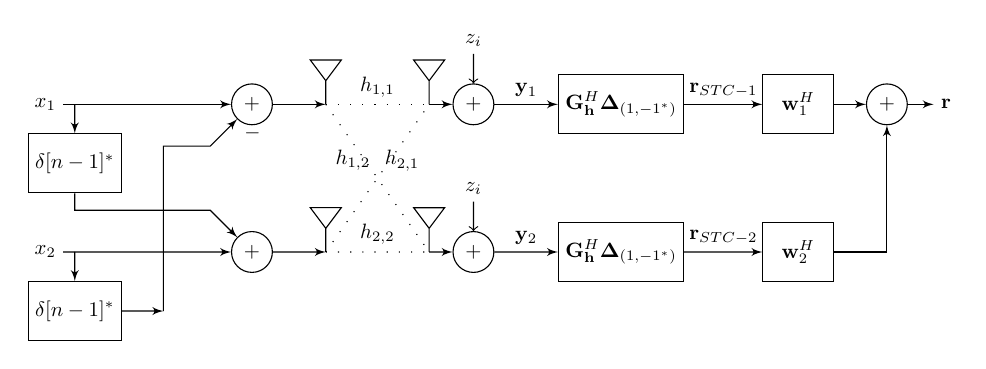
\begin{tikzpicture}[auto, node distance=2cm,>=latex', scale=0.75, every node/.style={scale=0.75}]
        \node [pinstyle, name=input1] {$x_1$};
        \node [pinstyle,below of=input1, node distance=2.5cm, name=input2] {$x_2$};        
        \node [coordinate,right of=input1,node distance=.5cm, name=split1] {};        
        \node [coordinate,right of=input2,node distance=.5cm, name=split2] {};
        \draw [draw,-,align=center] (input1) -- (split1);
        \draw [draw,-,align=center] (input2) -- (split2);
        \node [block,below of=split1, node distance=1cm] (del1) {$\delta[n-1]^*$};
        \node [block,below of=split2, node distance=1cm] (del2) {$\delta[n-1]^*$};
        \draw [draw,->,align=center] (split1) -- (del1);        
        \draw [draw,->,align=center] (split2) -- (del2);     
        \node [sum, right of=split1, node distance=3cm] (sum1) {$+$};   
        \node [sum, right of=split2, node distance=3cm] (sum2) {$+$};   
        \draw [draw,->,align=center] (split1) -- (sum1);        
        \draw [draw,->,align=center] (split2) -- (sum2);  
        \node[coordinate] (s2d) at($(sum2)+(135:1)$) {};
        \draw [->] (del1) |- (s2d) --  (sum2);
        \node [coordinate,right of=del2, node distance=1.5cm] (corner) {};
        \draw [->] (del2) -- (corner);
        \node[coordinate] (s1d) at($(sum1)+(225:1)$) {};
        \draw [->] (corner) |- (s1d) -- node[pos=0.99,anchor=north west] {$-$} (sum1);
        \foreach \a in {1,2}{
            \node [input, right of=sum\a, node distance=1.25cm, name=txant\a] {};
            \node [input, right of=txant\a, node distance=1.75cm, name=rxant\a] {};
            \draw [draw] (txant\a) \antenna;
            \draw [draw,->,align=center] (sum\a) -- (txant\a);
%             \draw [draw,loosely dotted,-,align=center] (txant\a)  -- node {$h_\a^*$} (rxant1);
            \draw [draw] (rxant\a) \antenna;
            \node [sum, right of=rxant\a, node distance=.75cm, pin={[pinstyle, pin distance=.5cm]above:$z_i$}] (sumz\a) {$+$};
            \draw [draw,->,align=center] (rxant\a) -- (sumz\a);
            \node [block, right of=sumz\a, node distance=2.5cm, name=wf\a] {$\Gb_{\h}^H\Dl_{(1,-1^*)}$}; 
            \draw[->] (sumz\a) -- node {$\y_{\a}$} (wf\a);             
            \node [block, right of=wf\a, node distance=3cm, name=mrc\a] {$\w_\a^H$};
            \draw[->]  (wf\a) -- node {$\rr_{STC-\a}$} (mrc\a);             
            }
        \foreach \a in {1,2}{
            \foreach \b in {1,2}{
                \draw [draw,loosely dotted,-,align=center] (txant\a)  -- node {$h_{\b,\a}$} (rxant\b);
            }
        }
          \node [sum, right of=mrc1, node distance=1.5cm] (sumrc) {$+$};
            \draw[->]  (mrc1) -- (sumrc);             
            \draw[->]  (mrc2) -| (sumrc);             
        \node [pinstyle, right of=sumrc, node distance=1cm, name=output] {$\rr$};           
            \draw[->]  (sumrc) -- (output);   
        \end{tikzpicture}
\end{figure}
\begin{itemize}
 \item Alamoutti decoding $\rr_{STC-j}=\Gb_{\h}^H\Dl_{(1,-1^*)}\y_i=(|h_{j,1}|^2+|h_{j,2}|^2)\I\x =\|\h_j\|^2 \x$
 \item MRC $\rr=\left(\begin{array}{c}r_1\\r_2\end{array}\right)=\frac{(\|\h_1\|^2)^*}{\|\Hb\|}\rr_{STC-1}+\frac{(\|\h_2\|^2)^*}{\|\Hb\|}\rr_{STC-2}$
 \item Equivalent Channel $\rr=\frac{\|\Hb\|^2}{\sqrt{2}}\I_2\x+\z'\to$ Array gain $2\times$, Diversity $4\times$. 
\end{itemize}
}


\frame[allowframebreaks]{\frametitle{Transmitter Antenna Selection and MIMO}
\begin{columns}
 \begin{column}{7cm}    
 \begin{figure}
    \centering
    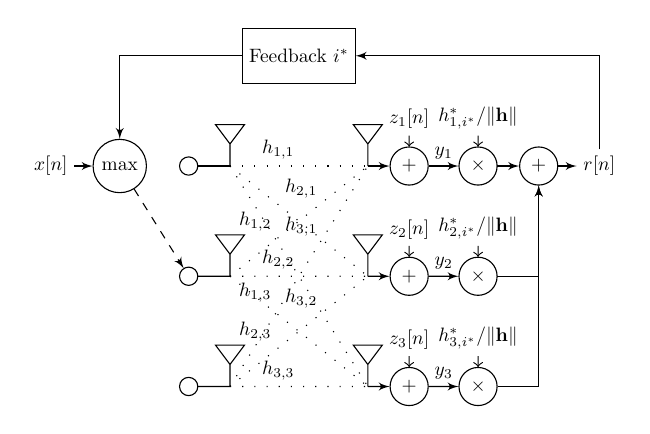
\begin{tikzpicture}[auto, node distance=2cm,>=latex', scale=0.7, every node/.style={scale=0.7}]
        \node [pinstyle, name=input1] {$x[n]$};
        \node [sum, right of=input1, name=split, node distance=1.25cm] {$\max$};
        \draw [draw,->,align=center] (input1) -- (split);        
            \node [sum,right of=split, node distance=1.25cm] (mult1) {};
        \foreach \a [evaluate=\a as \prev using int(\a-1)] in {2,3}{
            \node [sum,below of=mult\prev, node distance=2cm] (mult\a) {};  
        }
        \draw [draw,->,dashed,align=center] (split) -- (mult2);
        \foreach \a in {1,2,...,3}{
            \node [input, right of=mult\a, node distance=.75cm, name=txant\a] {};
            \draw [draw] (txant\a) \antenna;
            \draw [draw,-,align=center] (mult\a) -- (txant\a);
            }
        \foreach \a in {1,2,...,3}{
            \node [input, right of=txant\a, node distance=2.5cm, name=rxant\a] {}; 
            \draw [draw] (rxant\a) \antenna;
            \node [sum, right of=rxant\a, node distance=.75cm, pin={[pinstyle,pin distance=.2cm]above:$z_\a[n]$}] (sum\a) {$+$};
            \draw [draw,->,align=center] (rxant\a) -- (sum\a);
            \node [sum,right of=sum\a, node distance=1.25cm, pin={[pinstyle, pin distance=.2cm]above:$h_{\a,i^*}^*/\|\h\|$}] (mult\a) {$\times$};
            \draw [draw,->,align=center] (sum\a) -- node {$y_\a$} (mult\a);
%             \noce [block, right of=sum\a, node distance=1cm] (weight\a) {$w_\a$};
%             \draw [draw,->,align=center] (sum\a) -- (weight\a);
        }
        \foreach \a in {1,2,...,3}{
            \foreach \b in {1,2,...,3}{
                \draw [draw,loosely dotted,-,align=center] (txant\a)  -- node[pos=.35] {$h_{\b,\a}$} (rxant\b);
            }
        }
        \node [sum, right of=mult1, name=sumacc, node distance=1.1cm] {$+$};
        \draw [draw,->,align=center] (mult1) -- (sumacc);
        \foreach \a in {2,3}{
            \draw [draw,->,align=center] (mult\a) -| (sumacc);
        }
        \node [pinstyle, right of=sumacc, node distance=1.1cm, name=output] {$r[n]$};
        \draw[->] (sumacc) -- (output);
    \node[block] (fb) at ($(txant1)!.5!(rxant1)+(0,2)$) {Feedback $i^*$};
    \draw[->] (output) |- (fb);
    \draw[->] (fb) -| (split);
        \end{tikzpicture}
\end{figure}

 \end{column}
 \begin{column}{5cm}    
$$\rho=\frac{P}{\sigma_z^2}\max_{i\in\{1\dots N_{t}\}}\left(\sum_{j=1}^{N_{r}}|h_{j_i}|^2\right)$$
$$f(\frac{\rho}{P/\sigma_z^2})\sim\max\textnormal{-}N_{t}\textnormal{-}\frac{1}{\sqrt{2}}\chi^2(2N_{r})$$
\begin{itemize}
 \item Array Gain $$\overline{\rho}=\left(\sum_{k=1}^{N_{t}}{N_{t} \choose k}\frac{(1)^{k-1}}{k}\right)\frac{N_{r}P}{\sigma_z^2}$$
 \item Diversity $$P_o\approx\overline{\rho}^{-N_{r}N_{t}}$$
\end{itemize}
 \end{column}
\end{columns}
}

\frame[allowframebreaks]{\frametitle{Multiple Antenna Selection and MIMO}
\textcolor{VCobalt}{Intuition of DMT}
\begin{columns}
\begin{column}{6cm}
\begin{itemize}
\item Choose $M$ largest $|h_{i,j}|^2$
\item \textbf{Different column and row}
\item $(N_{r}-1)(N_{t}-1)$ choices
\end{itemize}

 $$\Hb=\left(\begin{array}{cccc}
              h_{1,1}&h_{1,2}&h_{1,3}\\
              h_{2,1}&h_{2,2}&h_{2,3}\\
              h_{3,1}&h_{3,2}&h_{3,3}\\
              h_{4,1}&h_{4,2}&h_{4,3}\\
             \end{array}\right)$$
 $$\|\Hb\|^2=|h_{1,1}|^2+\dots+|h_{1,3}|^2\dots+|h_{4,3}|^2$$
\end{column}

\begin{column}{6cm}
\begin{itemize}
\item $M=1$
\begin{itemize}
\item 1 row, 1 column
\item Last choice $4\times 3$ polar
\end{itemize}
\item $M=2$
\begin{itemize}
\item 2 rows, 2 columns
\item Last choice  $3\times 2$
\end{itemize}
\item $M=3$
\begin{itemize}
\item 3 rows, 3 columns 
\item Last choice $2\times 1$
\end{itemize}
\end{itemize}
 
\end{column}
\end{columns}

\pagebreak
\begin{columns}
 \begin{column}{6.5cm}    
 \begin{figure}
    \centering
    \caption{Another Intuition of DMT}
    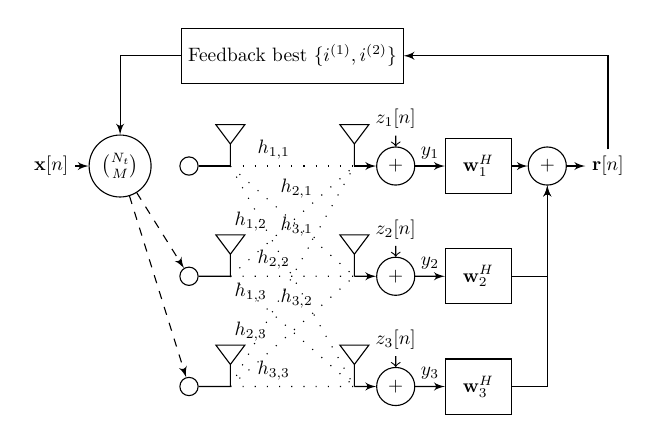
\begin{tikzpicture}[auto, node distance=2cm,>=latex', scale=0.7, every node/.style={scale=0.7}]
        \node [pinstyle, name=input1] {$\x[n]$};
        \node [sum, right of=input1, name=split, node distance=1.25cm] {${N_{t} \choose M}$};
        \draw [draw,->,align=center] (input1) -- (split);        
            \node [sum,right of=split, node distance=1.25cm] (mult1) {};
        \foreach \a [evaluate=\a as \prev using int(\a-1)] in {2,3}{
            \node [sum,below of=mult\prev, node distance=2cm] (mult\a) {};  
        }
        \draw [draw,->,dashed,align=center] (split) -- (mult2);
        \draw [draw,->,dashed,align=center] (split) -- (mult3);
        \foreach \a in {1,2,...,3}{
            \node [input, right of=mult\a, node distance=.75cm, name=txant\a] {};
            \draw [draw] (txant\a) \antenna;
            \draw [draw,-,align=center] (mult\a) -- (txant\a);
            }
        \foreach \a in {1,2,...,3}{
            \node [input, right of=txant\a, node distance=2.25cm, name=rxant\a] {}; 
            \draw [draw] (rxant\a) \antenna;
            \node [sum, right of=rxant\a, node distance=.75cm, pin={[pinstyle,pin distance=.2cm]above:$z_\a[n]$}] (sum\a) {$+$};
            \draw [draw,->,align=center] (rxant\a) -- (sum\a);
            \node [block,right of=sum\a, node distance=1.5cm] (mult\a) {$\w_\a^H$};
            \draw [draw,->,align=center] (sum\a) -- node {$y_\a$} (mult\a);
%             \noce [block, right of=sum\a, node distance=1cm] (weight\a) {$w_\a$};
%             \draw [draw,->,align=center] (sum\a) -- (weight\a);
        }
        \foreach \a in {1,2,...,3}{
            \foreach \b in {1,2,...,3}{
                \draw [draw,loosely dotted,-,align=center] (txant\a)  -- node[pos=.35] {$h_{\b,\a}$} (rxant\b);
            }
        }
        \node [sum, right of=mult1, name=sumacc, node distance=1.25cm] {$+$};
        \draw [draw,->,align=center] (mult1) -- (sumacc);
        \foreach \a in {2,3}{
            \draw [draw,->,align=center] (mult\a) -| (sumacc);
        }
        \node [pinstyle, right of=sumacc, node distance=1.1cm, name=output] {$\rr[n]$};
        \draw[->] (sumacc) -- (output);
    \node[block] (fb) at ($(txant1)!.5!(rxant1)+(0,2)$) {Feedback best $\{i^{(1)},i^{(2)}\}$};
    \draw[->] (output) |- (fb);
    \draw[->] (fb) -| (split);
        \end{tikzpicture}
\end{figure}

 \end{column}
 \begin{column}{6cm}    
\begin{itemize}
\item Matrix Columns
    $$\Hb=\left[\h_1|\h_2|\dots|\h_{N_{r}}\right]$$
\item Choose $M$ largest $\|\h_i\|^2$
\begin{itemize}
    \item Diversity $(N_{t}-M)$
\end{itemize}
\item Linear Receiver
    $$\W^H=\left[\begin{array}{c}\w_1^H\\\hline\w_2^H\\\hline\vdots\\\hline \w_{M}^H\end{array}\right]$$
    \vspace{-.1in}
    \begin{itemize}
     \item ZF $M-1$ ISI terms
     \item Leftover array gain $(N_{r}-M)$
    \end{itemize}
\end{itemize}
 \end{column}
\end{columns}
}

\frame[allowframebreaks]{\frametitle{Limited Feedback MIMO}

 \begin{figure}
    \centering
    \caption{Limited Feedback Precoding}
    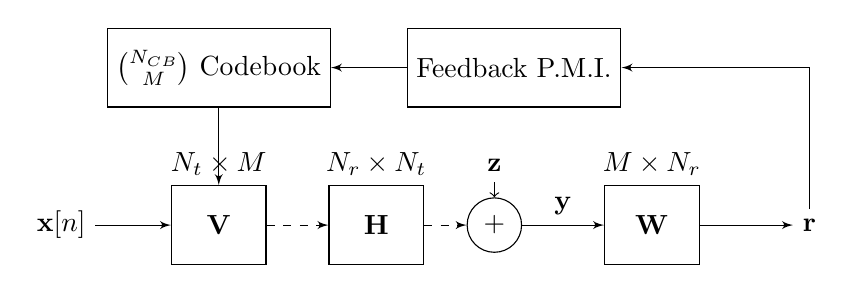
\begin{tikzpicture}[auto, node distance=2cm,>=latex']%, scale=0.7, every node/.style={scale=0.7}]
        \node [pinstyle, name=input] {$\x[n]$};
        \node [block, right of=input, name=precod,label={$N_{t}\times M$}] {$\V$};        
        \draw [->] (input) -- (precod);
        \node [block, right of= precod, name=ch,label={$N_{r}\times N_{t}$}] {$\Hb$};
        \draw [->,dashed] (precod) -- (ch);
        \node [sum, right of= ch, node distance=1.5cm, pin={[pinstyle,pin distance=.2cm]above:$\z$}] (sumz) {$+$};
        \draw [->,dashed] (ch) -- (sumz);
        \node [block, right of= sumz, name=wf,label={$M\times N_{r}$}] {$\W$};
        \draw [->] (sumz) -- node {$\y$} (wf);
        \node [pinstyle, right of=wf, name=output] {$\rr$};
        \draw[->] (wf) -- (output);
        \node[block] (fb) at ($(ch)!.5!(wf)+(0,2cm)$) {Feedback P.M.I.};
        \draw[->] (output) |- (fb);
        \node[block, above of = precod] (cb) {${N_{CB} \choose M}$ Codebook};
        \draw[->] (fb) -- (cb);
        \draw[->] (cb) -- (precod);
        \end{tikzpicture}
\end{figure}
\begin{definition}[Precoding Codebook]
 A finite collection of several \textbf{possible} precoding matrices
  $$\mathcal{V}_{CB}=\left\{\V_1,\V_2|\dots|\V_{_{CB}}\right\},\textnormal{ where }\V_i\in\mathbb{C}^{N_{t}\times M}$$
\end{definition}

 
\pagebreak
 \begin{itemize}
  \item When matrix $\V_i\in \mathcal{V}_{CB}$ is selected, the equivalent channel is
    $$\rr=\underset{M\times N_{r}}{\W}\underset{N_{r}\times N_{t}}{\Hb}\underset{N_{t}\times M}{\V_i}\x+\z$$  
  \item Admits MF/ZF/MMSE linear and non-linear receiver 
    $$\W=(\V_i^H\Hb^H\Hb\V_i+\frac{\sigma_z^2}{P}\I_{M})\V_i^H\Hb^H$$
 \end{itemize}
\begin{definition}[Precoding Matrix Indicator]
The receiver knows $\Hb$, computes a prediction of performance for all $\V_i\in \mathcal{V}_{CB}$, and reports the best $i^*$ to the transmitter.
\end{definition}
 
 
\pagebreak
 \begin{itemize}
  \item Example: for MMSE linear $\W$, $\V_i$ for maximum SINR is
  $$\V_i^*=\arg \max_{\V_i\in\mathcal{V}_{CB}} \mathrm{SINR}(\V_i)=\arg \max_{\V_i\in\mathcal{V}_{CB}}\frac{P}{\sigma_z^2\left(\sum_{i=1}^{M}\frac{1}{\lambda_i(\Hb\V_i)+\frac{M\sigma_z^2}{P}}\right)}$$  
  \item Example: $M=1$, Tx. Antenna Selection and MRC in this notation
  $$\mathcal{V}=\left\{\left(\begin{array}{c}1\\0\\\vdots\\0\end{array}\right),\left(\begin{array}{c}0\\1\\\vdots\\0\end{array}\right),\dots,\left(\begin{array}{c}0\\0\\\vdots\\1\end{array}\right)\right\}\qquad \W=\frac{\h_{i^*}^H}{\|\h_{i^*}\|}$$
  \pagebreak
  \item Example: $M=1$, LOS Beamforming Codebook with Limited Feedback
       $$\mathcal{V}=\left\{\vv(0^o),\vv(45^o)\dots\right\}$$

 \begin{columns}
  \begin{column}{6cm}    
    \begin{figure}
    \centering
    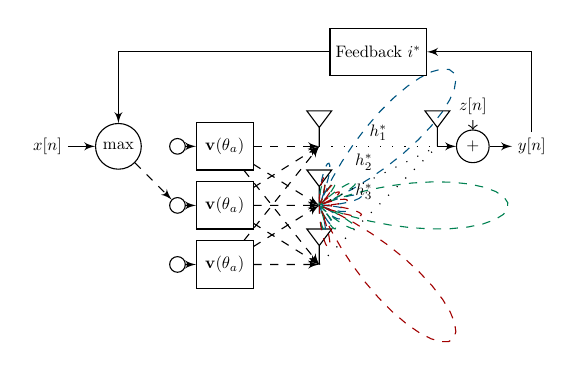
\begin{tikzpicture}[auto, node distance=2cm,>=latex', scale=0.6, every node/.style={scale=0.6}]
        \tikzmath{
        function ULA(\x) {
            if abs(\x) < 0.001 then {
                return 4.0;
            } else {
                return abs(sin(deg(pi*\x/2*8) )/sin(deg(pi/2*\x)))/sqrt(4);
            };
        };
    }
        \node [pinstyle, name=input1] {$x[n]$};
        \node [sum, right of=input1, name=split, node distance=1.5cm] {$\max$};
        \draw [draw,->,align=center] (input1) -- (split);        
            \node [sum,right of=split, node distance=1.25cm] (mult1) {};
        \foreach \a [evaluate=\a as \prev using int(\a-1)] in {2,3}{
            \node [sum,below of=mult\prev, node distance=1.25cm] (mult\a) {};  
        }
        \draw [draw,->,dashed,align=center] (split) -- (mult2);              
        \foreach \a in {1,2,...,3}{
            \node [block, right of=mult\a, node distance=1cm, name=beamv\a] {$\vv(\theta_a)$};
            \draw [draw,->,align=center] (mult\a) -- (beamv\a);
            }
        \foreach \a in {1,2,...,3}{
            \node [input, right of=beamv\a, node distance=2cm, name=txant\a] {};
            \draw [draw] (txant\a) \antenna;
            
            \foreach \b in {1,2,...,3}{
                \draw [draw,dashed,->,align=center] (beamv\b) -- (txant\a);
            }
            }
        \node [input, right of=txant1, node distance=2.5cm, name=rxant1] {};        
        \draw[domain=-1:1, samples=100, VCobalt, dashed, shift=(txant2)] plot ({ULA(\x-.5 )*cos(deg(\x*pi/2))}, {ULA(\x-.5)*sin(deg(\x*pi/2))}); 
        \draw[domain=-1:1, samples=100, KYJade, dashed, shift=(txant2)] plot ({ULA(\x )*cos(deg(\x*pi/2))}, {ULA(\x)*sin(deg(\x*pi/2))}); 
        \draw[domain=-1:1, samples=100, ARust, dashed, shift=(txant2)] plot ({ULA(\x+.5 )*cos(deg(\x*pi/2))}, {ULA(\x+.5)*sin(deg(\x*pi/2))}); 
        \foreach \a [evaluate=\a as \prev using int(\a-1)] in {1,2,3}{
            \draw [draw,loosely dotted,-,align=center] (txant\a)  -- node {$h_\a^*$} (rxant1);
            }
            \draw [draw] (rxant1) \antenna;
    \node [sum, right of=rxant1, node distance=.75cm, pin={[pinstyle, pin distance=.2cm]above:$z[n]$}] (sumacc) {$+$};
    \draw [draw,->,align=center] (rxant1) -- (sumacc);
    \node [pinstyle, right of=sumacc, node distance=1.25cm, name=output] {$y[n]$};
    \draw[->] (sumacc) -- (output);
    \node[block] (fb) at ($(txant1)!.5!(rxant1)+(0,2)$) {Feedback $i^*$};
    \draw[->] (output) |- (fb);
    \draw[->] (fb) -| (split);
        \end{tikzpicture}
%   
\end{figure}
  \end{column}
  \begin{column}{6cm}
  \begin{itemize}
   \item LOS BF $\vv(\theta)=\left(\begin{array}{c}e^{j\pi 0\times \cos(\theta)}\\e^{j\pi 1\times\cos(\theta)}\\\vdots\\e^{j\pi (N_{t}-1)\times\cos(\theta)}\end{array}\right)$\\ \ \\
   \item $\mathcal{V}$ as matrix columns $\V_{CB} =\left[\vv(\theta_1)|\vv(\theta_2)|\dots|\vv(\theta_{N_{CB}})\right]$\\ \ \\
   \item \textbf{Sector-Antenna selection} over the columns of $\Hb\V_{CB}$
  \end{itemize}
  \end{column}
 \end{columns}
  \end{itemize}
}

\frame{\frametitle{Representation of the Channel in Angle-Domain}
 \begin{itemize}
   \item Design Transmit And Receive Beam Codebooks
   $$\V_{CB} =\left[\vv_1|\vv_2|\dots|\vv_{N_{CB-t}}\right],\qquad \W_{CB} =\left[\w_1|\w_2|\dots|\w_{N_{CB-r}}\right]$$
   \item Equivalent channel matrix 
   $$\tiny \A = \W^H\Hb\V=\left(\begin{array}{cccc}                   
a_{1,1}&a_{1,2}&\dots&a_{1,N_{CB-t}}\\                   
a_{2,1}&a_{1,2}&\dots&a_{2,N_{CB-t}}\\                   
\vdots&\vdots&\ddots&\vdots\\                   
a_{N_{CB-r},1}&a_{N_{CB-r},2}&\dots&a_{N_{CB-r},N_{CB-t}}\\
                  \end{array}\right)$$
   \item Apply all known techniques to equivalent channel 
   $$\rr=\A\s+\z'\textnormal{ where } \z'=\W\z$$
    \begin{itemize}
    \item Transmitted power constraint $\to$ $\|\vv_{i}\|^2=1$ $\to$ $\Ex{}{\|\x\|^2}=\Ex{}{\|\s\|^2}=P$
    \item Received noise power $\to$ $\|\w_{i}\|^2=1$ $\to$ $\Ex{}{\|\z'\|^2}=\Ex{}{\|\W_{\mathcal{R}}\z\|^2}=M\sigma_z^2$
    \end{itemize}
  \end{itemize}
  }
  
\frame{\frametitle{Beam Steering}
  
   $$r[n]=a_{i,j}s[n]+z'[n]=\w_{j}\Hb\vv_i s[n]+z'[n]\textnormal{ where } i,j=\arg\max |a_{i,j}|^2$$
    \begin{figure}
    \centering
    \caption{Equivalent Transmit+Receive Antenna Selection}
    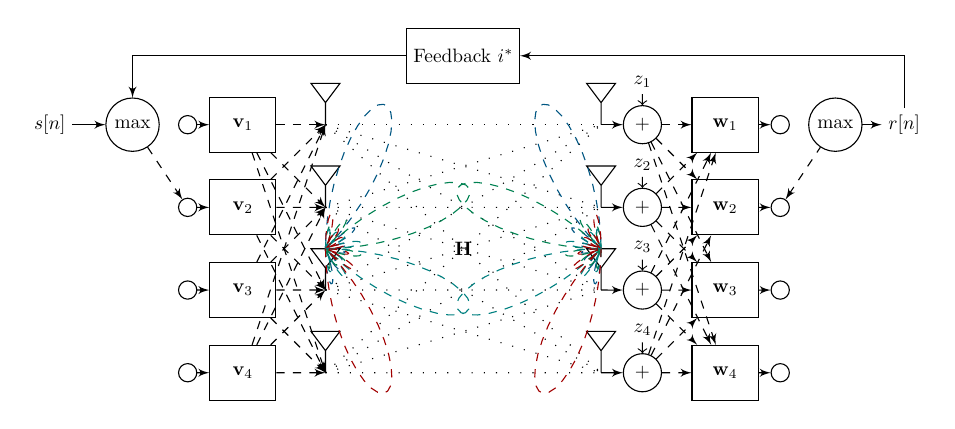
\begin{tikzpicture}[auto, node distance=2cm,>=latex', scale=0.7, every node/.style={scale=0.7}]
        \tikzmath{
        function ULA(\x) {
            if abs(\x) < 0.001 then {
                return 2.0;
            } else {
                return abs(sin(deg(pi*\x/2*8) )/sin(deg(pi/2*\x)))/sqrt(8);
            };
        };
    }
        \node [pinstyle, name=input1] {$s[n]$};
        \node [sum, right of=input1, name=split, node distance=1.5cm] {$\max$};
        \draw [draw,->,align=center] (input1) -- (split);        
            \node [sum,right of=split, node distance=1cm] (pint1) {};
        \foreach \a [evaluate=\a as \prev using int(\a-1)] in {2,3,4}{
            \node [sum,below of=pint\prev, node distance=1.5cm] (pint\a) {};  
        }
        \draw [draw,->,dashed,align=center] (split) -- (pint2);              
        \foreach \a in {1,2,...,4}{
            \node [block, right of=pint\a, node distance=1cm, name=beamv\a] {$\vv_\a$};
            \draw [draw,->,align=center] (pint\a) -- (beamv\a);
            \node [input, right of=beamv\a, node distance=1.5cm, name=txant\a] {};
            \draw [draw] (txant\a) \antenna;
            \node [input, right of=txant\a, node distance=5cm, name=rxant\a] {};
            \draw [draw] (rxant\a) \antenna;
            \node [sum, right of=rxant\a, node distance=.75cm, pin={[pinstyle,pin distance=.2cm]above:$z_\a$}] (sum\a) {$+$};
            \draw [draw,->,align=center] (rxant\a) -- (sum\a);
            \node [block, right of=sum\a, node distance=1.5cm] (beamw\a) {$\w_\a$};  
            \node [sum,right of=beamw\a, node distance=1cm] (pinr\a) {};
            \draw [draw,->,align=center] (beamw\a) -- (pinr\a);       
            }
                 
        \foreach \a in {1,2,...,4}{      
            \foreach \b in {1,2,...,4}{
                \draw [draw,dashed,->,align=center] (beamv\b) -- (txant\a);
                \draw [draw,loosely dotted,-,align=center] (txant\a)  -- (rxant\b);
                \draw [draw,dashed,->,align=center] (sum\b) -- (beamw\a);   
            }      
        }
        \node at ($(txant2)!.5!(rxant3)$) {$\Hb$}; 
        \draw[domain=-1:1, samples=100, VCobalt, dashed, shift=($(txant2)!.5!(txant3)$)] plot ({ULA(\x-.75 )*cos(deg(\x*pi/2))}, {ULA(\x-.75)*sin(deg(\x*pi/2))}); 
        \draw[domain=-1:1, samples=100, KYJade, dashed, shift=($(txant2)!.5!(txant3)$)] plot ({ULA(\x-.25 )*cos(deg(\x*pi/2))}, {ULA(\x-.25)*sin(deg(\x*pi/2))}); 
        \draw[domain=-1:1, samples=100, TZTeal, dashed, shift=($(txant2)!.5!(txant3)$)] plot ({ULA(\x+.25 )*cos(deg(\x*pi/2))}, {ULA(\x+.25)*sin(deg(\x*pi/2))}); 
        \draw[domain=-1:1, samples=100, ARust, dashed, shift=($(txant2)!.5!(txant3)$)] plot ({ULA(\x+.75 )*cos(deg(\x*pi/2))}, {ULA(\x+.75)*sin(deg(\x*pi/2))}); 
        \draw[domain=-1:1, samples=100, VCobalt, dashed, shift=($(rxant2)!.5!(rxant3)$)] plot ({-ULA(\x-.75 )*cos(deg(\x*pi/2))}, {ULA(\x-.75)*sin(deg(\x*pi/2))}); 
        \draw[domain=-1:1, samples=100, KYJade, dashed, shift=($(rxant2)!.5!(rxant3)$)] plot ({-ULA(\x-.25 )*cos(deg(\x*pi/2))}, {ULA(\x-.25)*sin(deg(\x*pi/2))}); 
        \draw[domain=-1:1, samples=100, TZTeal, dashed, shift=($(rxant2)!.5!(rxant3)$)] plot ({-ULA(\x+.25 )*cos(deg(\x*pi/2))}, {ULA(\x+.25)*sin(deg(\x*pi/2))}); 
        \draw[domain=-1:1, samples=100, ARust, dashed, shift=($(rxant2)!.5!(rxant3)$)] plot ({-ULA(\x+.75 )*cos(deg(\x*pi/2))}, {ULA(\x+.75)*sin(deg(\x*pi/2))}); 
        \node [sum, right of=pinr1, name=sumacc] {$\max$};
        \draw [draw,<-,dashed,align=center] (pinr2) -- (sumacc);
        \node [pinstyle, right of=sumacc, node distance=1.25cm, name=output] {$r[n]$};
        \draw[->] (sumacc) -- (output);
        \node[block] (fb) at ($(txant1)!.5!(rxant1)+(0,1.25)$) {Feedback $i^*$};
        \draw[->] (output) |- (fb);
        \draw[->] (fb) -| (split);
        \end{tikzpicture}
\end{figure}
}

\frame{\frametitle{Hybrid Beamforming}
  
   $$\rr[n]=\A_{\mathcal{R},\mathcal{T}}\s[n]+\z'[n]=\W_{\mathcal{R}}\Hb\V_{\mathcal{T}} \s[n]+\z'[n],$$
   $$ \mathcal{R},\mathcal{T}=\arg\max_{\texttt{rows}(\A)\times\texttt{cols}(\A)} \|\A_{\mathcal{R},\mathcal{T}}\|^2$$
    \begin{figure}
    \centering
    \caption{Transmit+Receive Multiple-Equivalent-Antenna Selection}
    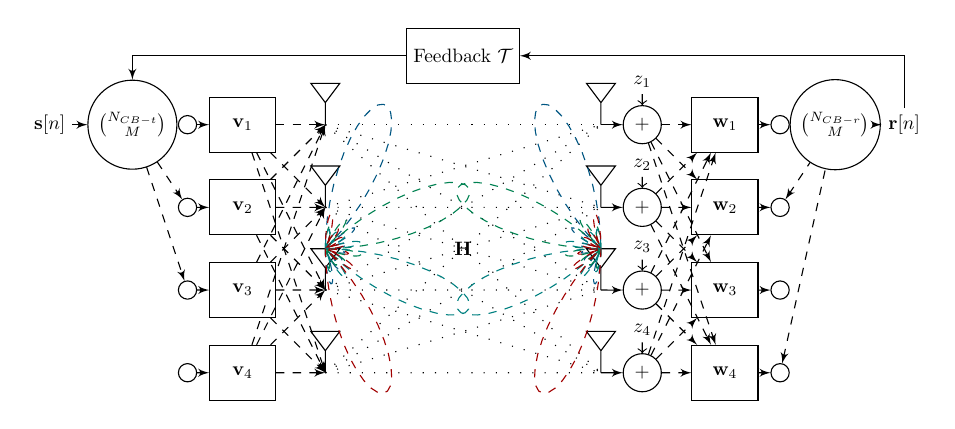
\begin{tikzpicture}[auto, node distance=2cm,>=latex', scale=0.7, every node/.style={scale=0.7}]
        \tikzmath{
        function ULA(\x) {
            if abs(\x) < 0.001 then {
                return 2.0;
            } else {
                return abs(sin(deg(pi*\x/2*8) )/sin(deg(pi/2*\x)))/sqrt(8);
            };
        };
    }
        \node [pinstyle, name=input1] {$\s[n]$};
        \node [sum, right of=input1, name=split, node distance=1.5cm] {${N_{CB-t} \choose M}$};
        \draw [draw,->,align=center] (input1) -- (split);        
            \node [sum,right of=split, node distance=1cm] (pint1) {};
        \foreach \a [evaluate=\a as \prev using int(\a-1)] in {2,3,4}{
            \node [sum,below of=pint\prev, node distance=1.5cm] (pint\a) {};  
        }
        \draw [draw,->,dashed,align=center] (split) -- (pint2);    
        \draw [draw,->,dashed,align=center] (split) -- (pint3);          
        \foreach \a in {1,2,...,4}{
            \node [block, right of=pint\a, node distance=1cm, name=beamv\a] {$\vv_\a$};
            \draw [draw,->,align=center] (pint\a) -- (beamv\a);
            \node [input, right of=beamv\a, node distance=1.5cm, name=txant\a] {};
            \draw [draw] (txant\a) \antenna;
            \node [input, right of=txant\a, node distance=5cm, name=rxant\a] {};
            \draw [draw] (rxant\a) \antenna;
            \node [sum, right of=rxant\a, node distance=.75cm, pin={[pinstyle,pin distance=.2cm]above:$z_\a$}] (sum\a) {$+$};
            \draw [draw,->,align=center] (rxant\a) -- (sum\a);
            \node [block, right of=sum\a, node distance=1.5cm] (beamw\a) {$\w_\a$};  
            \node [sum,right of=beamw\a, node distance=1cm] (pinr\a) {};
            \draw [draw,->,align=center] (beamw\a) -- (pinr\a);       
            }
                 
        \foreach \a in {1,2,...,4}{      
            \foreach \b in {1,2,...,4}{
                \draw [draw,dashed,->,align=center] (beamv\b) -- (txant\a);
                \draw [draw,loosely dotted,-,align=center] (txant\a)  -- (rxant\b);
                \draw [draw,dashed,->,align=center] (sum\b) -- (beamw\a);   
            }      
        }
        \node at ($(txant2)!.5!(rxant3)$) {$\Hb$}; 
        \draw[domain=-1:1, samples=100, VCobalt, dashed, shift=($(txant2)!.5!(txant3)$)] plot ({ULA(\x-.75 )*cos(deg(\x*pi/2))}, {ULA(\x-.75)*sin(deg(\x*pi/2))}); 
        \draw[domain=-1:1, samples=100, KYJade, dashed, shift=($(txant2)!.5!(txant3)$)] plot ({ULA(\x-.25 )*cos(deg(\x*pi/2))}, {ULA(\x-.25)*sin(deg(\x*pi/2))}); 
        \draw[domain=-1:1, samples=100, TZTeal, dashed, shift=($(txant2)!.5!(txant3)$)] plot ({ULA(\x+.25 )*cos(deg(\x*pi/2))}, {ULA(\x+.25)*sin(deg(\x*pi/2))}); 
        \draw[domain=-1:1, samples=100, ARust, dashed, shift=($(txant2)!.5!(txant3)$)] plot ({ULA(\x+.75 )*cos(deg(\x*pi/2))}, {ULA(\x+.75)*sin(deg(\x*pi/2))}); 
        \draw[domain=-1:1, samples=100, VCobalt, dashed, shift=($(rxant2)!.5!(rxant3)$)] plot ({-ULA(\x-.75 )*cos(deg(\x*pi/2))}, {ULA(\x-.75)*sin(deg(\x*pi/2))}); 
        \draw[domain=-1:1, samples=100, KYJade, dashed, shift=($(rxant2)!.5!(rxant3)$)] plot ({-ULA(\x-.25 )*cos(deg(\x*pi/2))}, {ULA(\x-.25)*sin(deg(\x*pi/2))}); 
        \draw[domain=-1:1, samples=100, TZTeal, dashed, shift=($(rxant2)!.5!(rxant3)$)] plot ({-ULA(\x+.25 )*cos(deg(\x*pi/2))}, {ULA(\x+.25)*sin(deg(\x*pi/2))}); 
        \draw[domain=-1:1, samples=100, ARust, dashed, shift=($(rxant2)!.5!(rxant3)$)] plot ({-ULA(\x+.75 )*cos(deg(\x*pi/2))}, {ULA(\x+.75)*sin(deg(\x*pi/2))}); 
        \node [sum, right of=pinr1, name=sumacc] {${N_{CB-r} \choose M}$};
        \draw [draw,<-,dashed,align=center] (pinr2) -- (sumacc);
        \draw [draw,<-,dashed,align=center] (pinr4) -- (sumacc);
        \node [pinstyle, right of=sumacc, node distance=1.25cm, name=output] {$\rr[n]$};
        \draw[->] (sumacc) -- (output);
        \node[block] (fb) at ($(txant1)!.5!(rxant1)+(0,1.25)$) {Feedback $\mathcal{T}$};
        \draw[->] (output) |- (fb);
        \draw[->] (fb) -| (split);
        \end{tikzpicture}
\end{figure}
}

\frame{\frametitle{Discrete Fourier Transform Codebook}
Matrix $\F_{K}$ with coefficients $F_{n,m}=\frac{1}{\sqrt{N_{CB}}}e^{-j2\pi\frac{nm}{N_{CB}}}$

\begin{columns}
 \begin{column}{6cm}
\begin{itemize}
\item Beams like LOS array
\begin{itemize}
\item Irregular angles and lobes
$$\theta_i=\{0,\acos(\frac{\pm 1}{2N_{CB}}),\acos(\frac{\pm 2}{2N_{CB}})\dots\}$$
\item Big sidelobes
\end{itemize}

\item Orthonormal matrix
  $$\F_{4}=\frac{1}{\sqrt{4}}\left(\begin{array}{cccc}
    1 & 1 & 1 & 1\\
    1 & -j & -1 & j\\
    1 & -1 & 1 & -1\\
    1 & j & -1 & -j\\
\end{array}\right)$$
\item FFT $O(\log(N_{CB}))$ complexity 
\begin{itemize}
\item Sometimes alt. $O(MN_{t})$
\end{itemize}
\end{itemize}
 \end{column}
 \begin{column}{6cm}
  \begin{figure}
   \centering
   \caption{$\theta_4=(0,30^o,90^o,-30^o)$}
   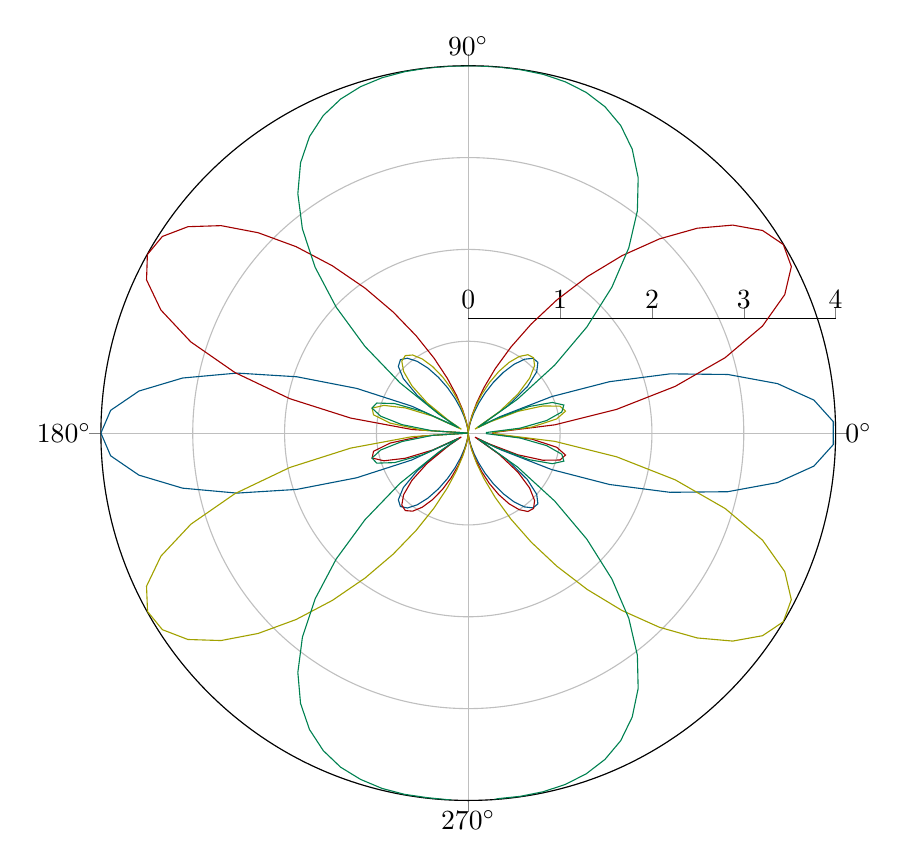
\begin{tikzpicture}
\begin{polaraxis}[
   xticklabel=$\pgfmathprintnumber{\tick}^\circ$,
   width=.9\columnwidth,
   height=.9\columnwidth,
   xtick={0,90,...,359},
   ytick={0,1,...,4},
   ymin=0, ymax=4,
   xticklabel style={anchor=180+\tick},
   yticklabel style={anchor=south, yshift=+.12\columnwidth},
   y axis line style={yshift=.12\columnwidth},
   ytick style={yshift=.12\columnwidth}
]
   \tikzmath{
        function ULA(\x) {
            if abs(\x) < .01 then {
                return 4.0;
            } else {
                return abs(sin(deg(pi/2*\x)*4 )/sin(deg(pi/2*\x)));
            };
        };
    }
\addplot [no markers, VCobalt,domain=-180:180,samples=100] {ULA(sin(x))};
\addplot [no markers, ARust,domain=-180:180,samples=100] {ULA(sin(x)-.5)};
\addplot [no markers, TAMustard,domain=-180:180,samples=100] {ULA(sin(x)+.5)};
\addplot [no markers, KYJade,domain=-180:180,samples=100] {ULA(sin(x)-1)};
\end{polaraxis}
\end{tikzpicture}
  \end{figure}
 \end{column} 
\end{columns}
}


\frame{\frametitle{Flat Sector Beamforming Codebook}
Matrix $\V_{CB}$ with coefficients designed by algorithms

\begin{columns}
 \begin{column}{6cm}
\begin{itemize}
\item Beams like Spatial Filter
\begin{itemize}
 \item Regular angles
    $$\theta_i=\{0,\pm 1\frac{\pi}{N_{CB}}),\pm 2\frac{\pi}{N_{CB}}\dots\}$$
 \item Flat rectangular sectors
 \item Small sidelobes
\end{itemize}
\item Unitary, not orthonormal
  $$\|\vv_i\|^2=1 \cancel{\Rightarrow} \V_{CB}^H\V_{CB}=\I_{N_{CB}}$$
\item Matrix product $O(N_{CB}N_{t})$
\begin{itemize}
\item Always simplified to $O(MN_{t})$
\end{itemize}
\end{itemize}
 \end{column}
 \begin{column}{6cm}
  \begin{figure}
   \centering
   \caption{$\theta_4=(0,45^o,90^o,-45^o)$}
   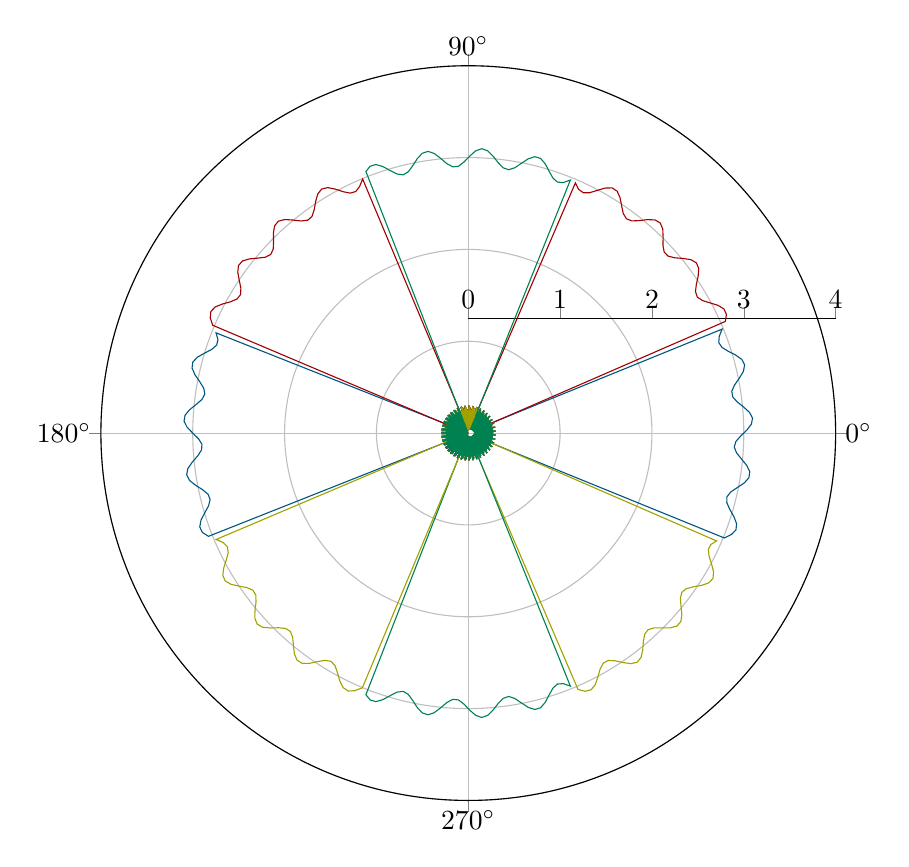
\begin{tikzpicture}
\begin{polaraxis}[
   xticklabel=$\pgfmathprintnumber{\tick}^\circ$,
   width=.9\columnwidth,
   height=.9\columnwidth,
   xtick={0,90,...,359},
   ytick={0,1,...,4},
   ymin=0, ymax=4,
   xticklabel style={anchor=180+\tick},
   yticklabel style={anchor=south, yshift=+.12\columnwidth},
   y axis line style={yshift=.12\columnwidth},
   ytick style={yshift=.12\columnwidth}
]
   \tikzmath{
        function flatBeam(\x) {
            if (abs(mod(\x+180,360)-180) < 22.5)  then {
                return abs(3+0.1*sin(32*x));
            } else {
                return abs(0.3*sin(64*x));
            };
        };
    }
\addplot [no markers, VCobalt,domain=-180:180,samples=300] {flatBeam(x)};
\addplot [no markers, ARust,domain=-180:180,samples=300] {flatBeam(x-45)};
\addplot [no markers, TAMustard,domain=-180:180,samples=300] {flatBeam(x+45)};
\addplot [no markers, KYJade,domain=-180:180,samples=300] {flatBeam(x+90)};
\addplot [no markers, VCobalt,domain=-180:180,samples=300] {flatBeam(180-x)};
\addplot [no markers, ARust,domain=-180:180,samples=300] {flatBeam(180-x-45)};
\addplot [no markers, TAMustard,domain=-180:180,samples=300] {flatBeam(180-x+45)};
\addplot [no markers, KYJade,domain=-180:180,samples=300] {flatBeam(180-x-90)};
\end{polaraxis}
\end{tikzpicture}
  \end{figure}
 \end{column} 
\end{columns}

}


\frame[allowframebreaks]{\frametitle{Statistical properties of Angular Channel}
\begin{theorem}[Correlated Gaussian Multiplication]
 If $\h$ is a White Gaussian vector, then $\ab=\W_{CB}\h$ is Gaussian with covariance
 $$\Sg_{\ab}=\Ex{}{\ab\ab^H}=\Ex{}{\W_{CB}\h\h^H\W_{CB}^H}=\W_{CB}\W_{CB}^H$$
\end{theorem}
\begin{definition}[Kroenecker Product]
 $$\W\odot\V=\left[\begin{array}{c|c|c}
 w_{1,1}\V&\dots&v_{1,N_{r}}\V\\\hline
 \vdots&\ddots&\vdots\\\hline
 w_{M,1}\V&\dots&h_{M,N_{r}}\V\\\hline
\end{array}\right],\;\to \textnormal{vec}(\W\Hb\V)=(\V^H\odot\W)\textnormal{vec}(\Hb)$$
\end{definition}
\pagebreak
\begin{itemize}
 \item Rich scattering ($N_{path}\gg N_{t}N_{r}$): I.i.d. Rayleigh $\A$ 
 \item Sparse Multipath  ($N_{path}\ll N_{t}N_{r}$): Low Rank $\A$ 
\end{itemize}


\begin{figure}
 \centering
 \caption{Average matrix $\Ex{}{\|\A\|^2}$ with 64-FFT CB}
 \subfigure[Rayleigh]{
    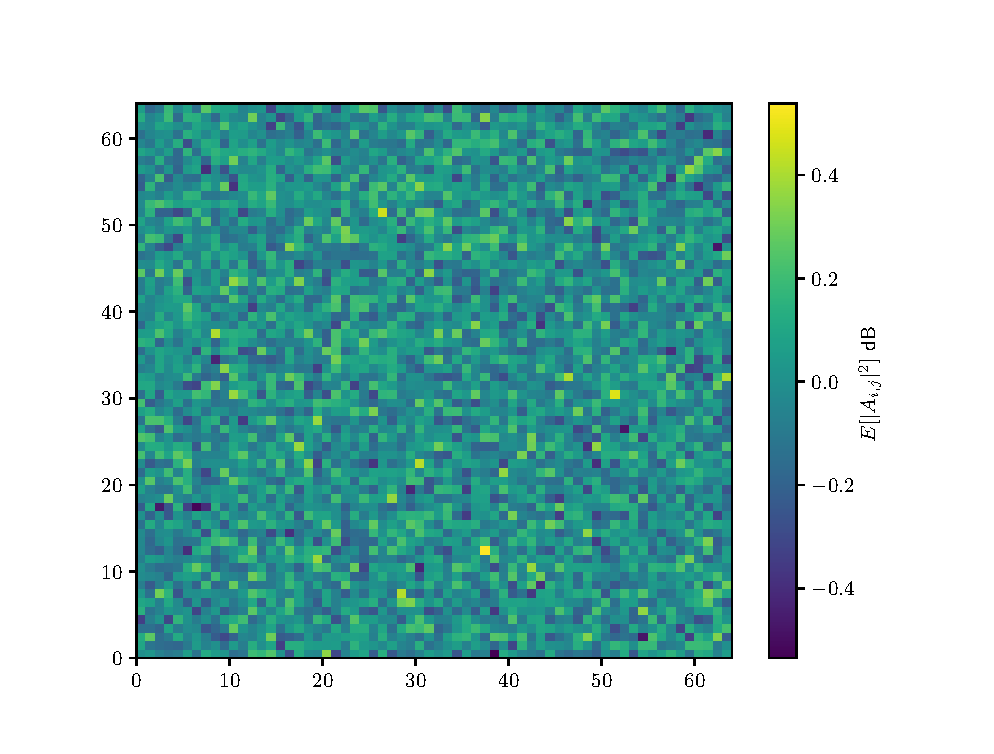
\includegraphics[width=.45\columnwidth]{AvgRayleighAmatrix}
 }
 \subfigure[3 Paths]{
    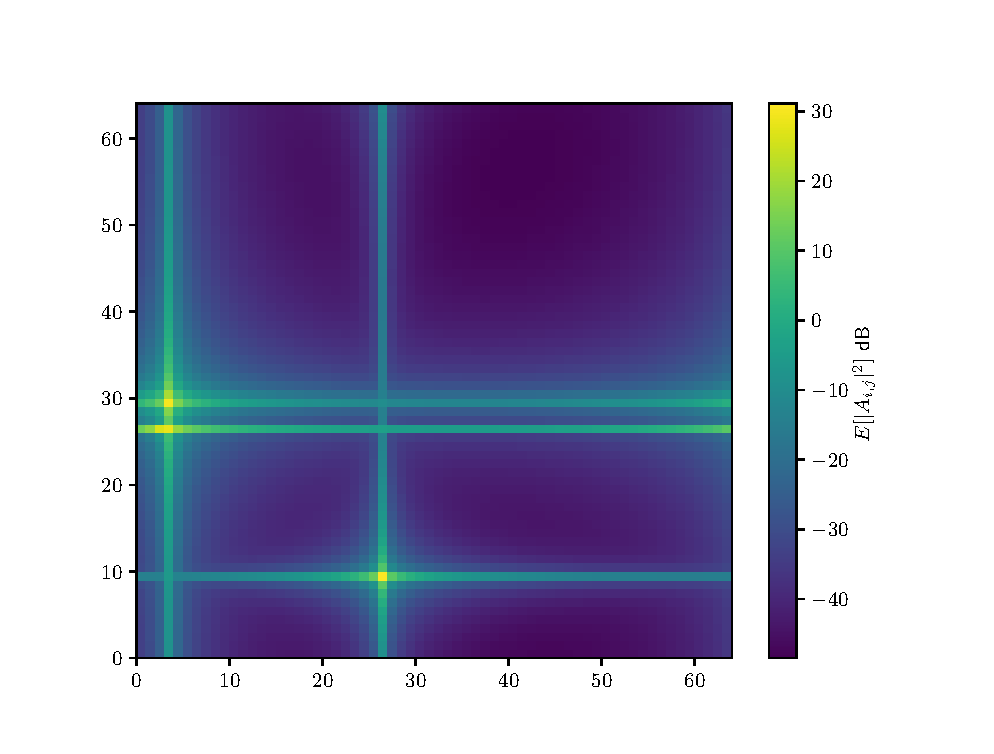
\includegraphics[width=.45\columnwidth]{AvgSparseAmatrix}
 }
\end{figure}

}


\frame[allowframebreaks]{\frametitle{Long-Term Beamforming}
\begin{definition}[Left and Right Covariance Matrices]
 Transmit antennas: $\Sg_{T}=\Ex{}{\Hb^H\Hb}$, Receive antennas: $\Sg_{R}=\Ex{}{\Hb\Hb^H}$
\end{definition}

\begin{itemize}
 \item I.i.d. vs correlated channel model
 $$\Hb=\Sg_{R}^{\frac{1}{2}}\Hb_{i.i.d.}\Sg_{T}^{\frac{1}{2}}\textnormal{ where } \Hb_{i.i.d.}\sim\mathcal{CN}(0,\sigma^2_h\I)$$
 \item Eigenvalue decomposition $\Sg_{T}=\V\Ld\V^H$, $\Sg_{R}=\U\Ld\U^H$
 $$\Hb=\U\Ld^{\frac{1}{2}}\Hb_{i.i.d.}\Ld^{\frac{1}{2}}\V$$
\end{itemize}

\begin{definition}[Long Term Stochastic Beamforming]
\begin{itemize}
 \item Same beam maintained over several block/fast fading realizations\\ \ \\
 \item Tx and Rx beams point to \textbf{covariance} largest eigenvalues\\ \ \\
\end{itemize}

 
\end{definition}


}

\end{document}


